\documentclass[11pt,a4paper]{article}

% ------------------------------------------------------------------
% Packages
% ------------------------------------------------------------------
\usepackage[utf8]{inputenc}
%\usepackage[T1]{fontenc}
\usepackage[margin=2.5cm]{geometry}
\usepackage{amsmath,amssymb,amsfonts}
\usepackage{graphicx}
\usepackage{booktabs}
\usepackage{multirow}
\usepackage{array}
\usepackage[table]{xcolor}
\usepackage{siunitx}
\usepackage{microtype}
\usepackage{enumitem}
\usepackage[authoryear,round]{natbib}
\usepackage{authblk}
\usepackage[skins,breakable]{tcolorbox}
\usepackage{caption}
\captionsetup{font=small,labelfont=bf}
\usepackage[colorlinks=true,linkcolor=blue!50!black,citecolor=blue!50!black,urlcolor=blue!50!black]{hyperref}
\usepackage[capitalise,noabbrev]{cleveref}

\sisetup{detect-all}
\graphicspath{{figures/}}

% "In plain words" boxes for non-specialist readers
\newtcolorbox{plainbox}[1][]{breakable,enhanced,colback=gray!6,colframe=gray!55,
  boxrule=0.5pt,arc=2pt,left=6pt,right=6pt,top=4pt,bottom=4pt,
  fonttitle=\bfseries\small,title={In plain words#1}}

\newcommand{\dd}{\mathrm{d}}
\newcommand{\kB}{k_{\mathrm{B}}}
\newcommand{\Href}{H_{\mathrm{ref}}}
\newcommand{\Tref}{T_{\mathrm{ref}}}
\newcommand{\rhyd}{r_{\mathrm{hyd}}}
\newcommand{\ours}{PINN-R}

% ------------------------------------------------------------------
\title{Physics-Informed Neural Networks for Reconstructing Missing Intervals in Martian Radio-Occultation Temperature and Pressure Profiles}

\author[1]{Shailendra Dabral}
\author[1]{Keshav Agrawal}
\affil[1]{Superplan\protect\\ \texttt{shailen@superplan.md}}
\date{}

\begin{document}
\maketitle

% ------------------------------------------------------------------
\begin{abstract}
Radio-occultation measurements from the Mars Reconnaissance Orbiter (MRO) give vertical profiles of temperature, pressure and number density in the lower Martian atmosphere, but parts of a profile can be missing or unreliable. We study how well such missing intervals can be filled in, and whether a \emph{physics-informed neural network} (PINN) --- a neural network trained to obey hydrostatic balance and the ideal-gas law --- does better than standard alternatives. Using 184 quality-controlled profiles from the MRO Radio Science (RSS) archive covering three Mars years, we hide contiguous intervals of 2, 5, 10 and 20\,km at the bottom, middle or top of 28 unseen test profiles (330 test cases) and compare twelve reconstruction methods: linear and monotone-cubic interpolation, hydrostatic integration of an interpolated temperature, a Gaussian process, empirical-orthogonal-function (EOF) optimal interpolation, a random forest, and data-only and physics-informed neural networks used with and without per-profile fine-tuning. The neural networks have identical architecture and training and differ only in the physics term. All hyper-parameters are chosen on separate validation profiles, and all comparisons use profile-level paired Wilcoxon tests with Holm correction. Our regularised, fine-tuned PINN reconstructs pressure with a mean relative error of 1.01\,\% (95\,\% CI 0.85--1.18\,\%) and number density with 1.92\,\% (1.55--2.32\,\%), significantly better than nine of eleven competitors for pressure and seven of eleven for density, including the identical data-only network (4.44\,\% and 5.10\,\%). For temperature its error of 3.00\,K is significantly lower than that of interpolation and the Gaussian process, but not significantly different from EOF optimal interpolation, which has the lowest temperature error (2.78\,K). Hydrostatic integration of an interpolated temperature remains a strong, physically exact competitor for pressure, especially inside interior gaps. The physics constraint reduces the hydrostatic residual of the network by an order of magnitude, makes it more robust to noisy inputs, and, after split-conformal calibration, yields predictive intervals with near-nominal coverage. The main lesson is that, in this setting, physics mainly fixes the \emph{thermodynamic consistency} of pressure and density, while temperature inside a gap is set by the statistical prior learned from other profiles.
\end{abstract}

\begin{plainbox}
Spacecraft orbiting Mars can measure how temperature and air pressure change with height by watching how a radio signal bends as it passes through the planet's thin atmosphere. Sometimes a stretch of that measurement is missing or unreliable, like a few missing rungs on a ladder. We tested twelve ways of ``filling in'' the missing rungs. One of them is a neural network (a flexible computer model that learns from examples) that is also forced to obey two simple laws of physics that every atmosphere follows. We found that this physics-aware network is very good at getting the \emph{pressure} and the \emph{air density} right --- usually within about 1--2\,\% --- and much better than an identical network that was not taught the physics. However, for \emph{temperature}, a well-established statistical method that learns typical temperature shapes from many past measurements does just as well or slightly better. In short: the physics keeps the numbers mutually consistent, but it cannot by itself tell you what the temperature was.
\end{plainbox}

\tableofcontents
\clearpage

% ==================================================================
\section{Introduction}\label{sec:intro}
% ==================================================================

\subsection{Why the vertical structure of the Martian atmosphere matters}
The Martian atmosphere is thin --- the surface pressure is less than one hundredth of that on Earth --- and is made mostly of carbon dioxide. Knowing how its temperature and pressure change with height is important for several reasons. Temperature profiles reveal how the atmosphere is heated by sunlight and dust, how it circulates, and where clouds of water ice or carbon-dioxide ice can form. Pressure and density profiles are needed to plan the entry, descent and landing of spacecraft and to understand how the atmosphere loses gas to space. Such profiles are also the ``ground truth'' against which numerical weather and climate models of Mars are tested.

\subsection{How radio occultation measures the atmosphere}
One of the most accurate ways to measure these profiles is \emph{radio occultation} \citep{fjeldbo1971,kursinski1997,hinson1999}. A spacecraft in orbit sends a very stable radio signal to Earth. As the spacecraft moves behind the planet (as seen from Earth), the signal passes through progressively deeper layers of the atmosphere before being cut off by the planet itself. The atmosphere acts like a weak lens and bends the signal slightly; this bending shows up as a tiny change in the frequency received on Earth. From the change in frequency over time one computes, layer by layer: (i) the bending angle of the ray, (ii) the refractive index of the air, (iii) the \emph{number density} of molecules (how many molecules per cubic metre), (iv) the \emph{pressure}, by adding up the weight of the air above each level, and finally (v) the \emph{temperature}, from the ideal-gas law. The result is a profile with a vertical resolution of a few hundred metres to about a kilometre, from the surface up to roughly 40\,km.

The Radio Science Subsystem (RSS) on NASA's Mars Reconnaissance Orbiter \citep{zurek2007} has produced many such profiles, and they are archived in NASA's Planetary Data System \citep{hinsonPDS}.

\begin{plainbox}
Imagine shining a laser pointer through the hot air above a road: the beam wobbles because warm and cool air bend light differently. Radio occultation uses the same idea with a radio beam and the Martian air. By measuring exactly how much the beam bends at each height, scientists can work out how many air molecules there are at that height, and from that the pressure and temperature.
\end{plainbox}

\subsection{The missing-data problem}
In practice, parts of a profile can be missing or unusable. Near the top, the retrieval has to start from an assumed temperature, so the first several kilometres carry large uncertainties. Near the surface, the signal can be distorted by sharp layers or by the terrain. Data dropouts and quality flags can remove intervals in between. Users of the data --- for example, people comparing profiles with a climate model or building a statistical average --- then face the question: \emph{what is the best estimate of temperature, pressure and density inside the missing interval, and how uncertain is that estimate?}

Classical answers include simply drawing a straight line or a smooth curve across the gap (interpolation), fitting a statistical model to the observed part of the same profile, or using statistics learned from many other profiles. A newer answer, which is the focus of this paper, is the physics-informed neural network.

\subsection{Physics-informed neural networks}
A neural network is a flexible mathematical function with many adjustable numbers (``weights'') that are tuned so that its outputs match training examples. A \emph{physics-informed neural network} (PINN) \citep{raissi2019,karniadakis2021} is trained not only to match the data but also to satisfy known physical equations. This is done by adding a penalty to the training objective whenever the network's outputs violate the equation. Because the equation can be checked at any point, including points where no data exist, PINNs can in principle use physics to guide predictions into data gaps.

For atmospheric profiles two laws are especially relevant: the \emph{ideal-gas law}, which links pressure, density and temperature, and \emph{hydrostatic balance}, which says that pressure at any height equals the weight of all the air above it. Both are explained in \cref{sec:physics}.

\subsection{An important subtlety}
The RSS retrieval itself \emph{uses} both of these laws to turn number density into pressure and temperature (\cref{sec:retrieval}). The reference data are therefore physically consistent by construction. This has two consequences that shape our study. First, when we report that a method is ``more hydrostatic'', we are measuring agreement with the physics that produced the reference, not the discovery of new physics. Second, and more importantly, hydrostatic balance relates the \emph{rate of change of pressure} to temperature, but it does not determine temperature itself. Inside a gap, temperature must come from somewhere else --- the observed data on either side and the typical shapes learned from other profiles. The strongest physics-based competitor is therefore not a data-only network but simply ``interpolate temperature, then integrate hydrostatic balance to get pressure'', and we include exactly this method as a baseline.

\subsection{Research questions and contributions}
We address five research questions:
\begin{description}[leftmargin=1.2cm,style=nextline]
\item[RQ1] \textbf{Accuracy.} Does a PINN reconstruct temperature, pressure and number density inside a contiguous missing interval more accurately than interpolation, a Gaussian process, hydrostatic integration, statistical climatologies and a data-only network with the same architecture and training?
\item[RQ2] \textbf{Where physics helps.} How does the benefit depend on the gap size (2--20\,km) and location (bottom, middle, top)? Middle gaps require interpolation; bottom and top gaps require extrapolation.
\item[RQ3] \textbf{Robustness.} How do methods degrade when the observed data are noisier than stated? How sensitive is the PINN to the weight given to the physics term?
\item[RQ4] \textbf{Uncertainty.} Are the predicted uncertainty ranges trustworthy (calibrated), and do larger predicted uncertainties correspond to larger errors?
\item[RQ5] \textbf{Generalisation.} Does a model trained on some Mars years transfer to an unseen Mars year?
\end{description}

Our contributions are:
\begin{enumerate}[leftmargin=*]
\item A careful, leakage-free benchmark for gap reconstruction in Martian radio-occultation profiles, with gaps defined in kilometres, profile-level train/validation/test splits, and hyper-parameters chosen only on validation profiles.
\item A PINN formulation in \emph{geopotential height} in which the ideal-gas law holds exactly by construction and hydrostatic balance enters as a dimensionless residual, removing ad-hoc scaling factors.
\item A regularised fine-tuning procedure (pulling weights toward a pre-trained ``climatological'' network) that adapts a single global network to each individual profile.
\item A comparison with eleven alternatives, including strong physically exact and statistical baselines, using paired non-parametric tests with multiple-comparison correction, uncertainty calibration via split-conformal prediction, and three additional robustness experiments.
\item An honest account of what physics does and does not contribute in this setting.
\end{enumerate}

\Cref{sec:physics} explains the physics, \cref{sec:data} the data, \cref{sec:design} the experimental design, \cref{sec:methods} all methods, \cref{sec:eval} the evaluation, \cref{sec:results} the results, \cref{sec:discussion} the discussion and limitations, and \cref{sec:conclusion} concludes. A glossary of terms is given in \cref{app:glossary}.

% ==================================================================
\section{Physical background}\label{sec:physics}
% ==================================================================

\subsection{The ideal-gas law}
For a gas whose molecules interact only weakly --- an excellent approximation for the thin Martian air --- pressure $P$, number density $n$ and temperature $T$ are linked by
\begin{equation}
P = n\,\kB\,T, \label{eq:idealgas}
\end{equation}
where $\kB = 1.380649\times10^{-23}\,\mathrm{J\,K^{-1}}$ is the Boltzmann constant. If two of the three quantities are known, the third follows.

\begin{plainbox}
Pressure is the push of molecules hitting a surface. More molecules (higher density) or faster molecules (higher temperature) give a bigger push. Equation~\eqref{eq:idealgas} says exactly how much bigger.
\end{plainbox}

\subsection{Hydrostatic balance and the scale height}
In an atmosphere at rest, the pressure at any level supports the weight of the air above it. Moving up a small height $\dd z$, the pressure drops by the weight of the thin slab of air that was left behind:
\begin{equation}
\frac{\dd P}{\dd z} = -\rho\, g = -n\, m\, g, \label{eq:hydro_z}
\end{equation}
where $\rho$ is mass density, $m$ the mean mass of one molecule and $g$ the gravitational acceleration. Dividing by $P$ and using \cref{eq:idealgas} gives
\begin{equation}
\frac{\dd \ln P}{\dd z} = -\frac{m g}{\kB T} \equiv -\frac{1}{H(T)},\qquad H(T) = \frac{\kB T}{m g}. \label{eq:scaleheight}
\end{equation}
$H$ is called the \emph{scale height}: over one scale height, pressure falls by a factor of $e\approx2.718$. On Mars, $H$ is about 10\,km. Note that \cref{eq:scaleheight} links the \emph{slope} of $\ln P$ to $T$; it does not say what $T$ is.

\begin{plainbox}
Climbing a mountain, the air gets thinner because there is less air above you pressing down. Hydrostatic balance is the rule that says how fast it thins: in warm air the pressure falls more slowly with height; in cold air it falls faster. On Mars, every 10\,km or so of height the pressure drops to about one-third.
\end{plainbox}

\subsection{Geopotential height}\label{sec:geopot}
Gravity on Mars is not exactly the same everywhere: it weakens with height, varies with latitude because the planet rotates and is slightly flattened, and has local irregularities. Using a simple $g=GM/r^2$ introduces errors of about 1.5\,\%. Instead we use the \emph{geopotential} $\Phi$ --- the gravitational (plus rotational) potential energy per unit mass relative to a reference surface --- which the RSS archive provides at every level, computed from a detailed gravity model. In terms of $\Phi$, hydrostatic balance is exact:
\begin{equation}
\frac{\dd\ln P}{\dd\Phi} = -\frac{m}{\kB T}.
\end{equation}
We define the \emph{geopotential height} $Z=\Phi/g_0$ with the conventional constant $g_0=3.71\,\mathrm{m\,s^{-2}}$, so that $Z$ has units of length and is close to the ordinary height. Then
\begin{equation}
\frac{\dd\ln P}{\dd Z} = -\frac{m g_0}{\kB T} = -\frac{1}{H(T)},\qquad H(T)=\frac{\kB T}{m g_0}. \label{eq:hydroZ}
\end{equation}
The choice of $g_0$ only rescales the coordinate and does not affect the physics. Because $\Phi$, latitude and longitude at each level follow from the observing geometry (not from the atmosphere), they are known even inside a data gap; using them as inputs does not leak any hidden information.

\subsection{How the retrieval uses the physics}\label{sec:retrieval}
The RSS retrieval proceeds as follows \citep{hinson1999}: bending angle $\rightarrow$ refractive index (via an Abel transform) $\rightarrow$ number density $n$ $\rightarrow$ pressure $P$ by integrating hydrostatic balance downward from the top $\rightarrow$ temperature $T=P/(n\kB)$. Hence the reference data satisfy \cref{eq:idealgas,eq:hydroZ} up to numerical precision. We verified this in a ``physics audit'' (\cref{sec:audit}).

% ==================================================================
\section{Data}\label{sec:data}
% ==================================================================

\subsection{Source}
We use the MRO RSS temperature--pressure profile product \texttt{MRO-M-RSS-5-TPS-V1.0} \citep{hinsonPDS}. Each row of the archive describes one height level of one profile and contains: profile identifier, Mars year, solar longitude $L_s$ (the season; $L_s=0^\circ$ is the northern spring equinox, $90^\circ$ northern summer solstice), planetocentric radius, latitude, longitude, geopotential, pressure and its 1$\sigma$ uncertainty $\sigma_P$, temperature and its uncertainty $\sigma_T$, and number density and its uncertainty $\sigma_n$. ``Mars year'' (MY) follows the standard convention in which MY\,1 began on 11 April 1955 \citep{clancy2000}; a Mars year lasts 687 Earth days.

\subsection{Pre-processing}
For each level we compute the geopotential height $Z$ (\cref{sec:geopot}), $\ln P$ and its uncertainty $\sigma_{\ln P}=\sigma_P/P$, and the sine and cosine of longitude and of $L_s$ (so that $359^\circ$ and $1^\circ$ are treated as close).

\subsection{Quality control}
Because each profile is retrieved downward from an assumed temperature at the top, $\sigma_T$ grows to about 10\,K near the top (\cref{fig:data}c). Results in the topmost kilometres would mainly reflect that initial assumption, not the atmosphere. We therefore removed all levels with $\sigma_T>5$\,K. We then kept only profiles whose geopotential increases strictly with height and which retain at least 40 levels. \Cref{tab:data} summarises the effect.

\begin{table}[t]
\centering\small
\caption{Data summary after quality control.}\label{tab:data}
\begin{tabular}{lr}
\toprule
Quantity & Value\\
\midrule
Profiles before / after quality control & 185 / 184\\
Height levels before / after quality control & 16\,686 / 13\,157\\
Median height trimmed from the top & 6.9\,km\\
Median vertical extent of a profile & 35.5\,km\\
Median number of levels per profile & 64\\
\midrule
Mars year 29: profiles, $L_s$ range & 65, $106.8^\circ$--$142.5^\circ$\\
Mars year 30: profiles, $L_s$ range & 46, $21.0^\circ$--$45.5^\circ$\\
Mars year 31: profiles, $L_s$ range & 73, $37.4^\circ$--$75.1^\circ$\\
\midrule
Implied mean molecular mass (median [IQR]) & 43.485 [43.483, 43.496]\,g\,mol$^{-1}$\\
Reference scale height $\Href$ at $\Tref=200$\,K & 10.31\,km\\
Max.\ relative deviation from ideal-gas law & $1.6\times10^{-5}$\\
Median hydrostatic residual of reference (RMS) & 0.0016\\
\bottomrule
\end{tabular}
\end{table}

\begin{figure}[t]
\centering
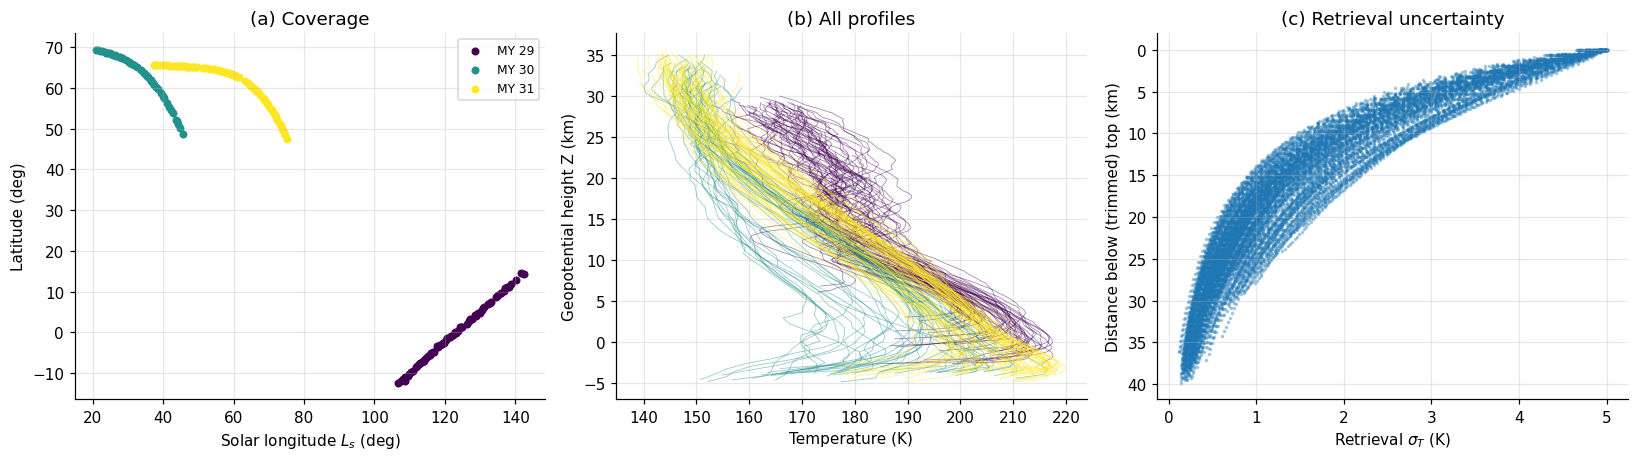
\includegraphics[width=\textwidth]{fig01_data_overview.png}
\caption{Overview of the data. (a) Season (solar longitude $L_s$) and latitude of each profile, coloured by Mars year (MY). Each Mars year covers a different season and latitude band. (b) All temperature profiles against geopotential height. (c) Retrieval temperature uncertainty $\sigma_T$ against distance below the (trimmed) top of each profile: uncertainty is largest near the top, where the retrieval is initialised.}
\label{fig:data}
\end{figure}

\subsection{Physics audit}\label{sec:audit}
Before using the data we checked that they satisfy the two laws.
\begin{itemize}[leftmargin=*]
\item \textbf{Ideal-gas law.} The largest relative deviation of $P/(n\kB T)$ from 1 over all 13\,157 levels is $1.6\times10^{-5}$, i.e.\ the law holds to rounding precision.
\item \textbf{Mean molecular mass.} Rearranging \cref{eq:hydroZ} between neighbouring levels gives the molecular mass $m$ assumed by the retrieval. Its median is 43.485\,g\,mol$^{-1}$, with an extremely narrow inter-quartile range (43.483--43.496), confirming a single constant was used. We adopt this value.
\item \textbf{Hydrostatic residual.} We define the dimensionless residual
\begin{equation}
\rhyd = \Href\,\frac{\dd\ln P}{\dd Z} + \frac{\Tref}{T},\qquad \Href=\frac{\kB\Tref}{m g_0}, \label{eq:rhyd}
\end{equation}
with $\Tref=200$\,K, giving $\Href=10.31$\,km. For exact balance, $\rhyd=0$; for typical errors it is of order one, so it needs no further scaling. Evaluated with finite differences on the reference data, the median RMS residual is 0.0016. This is the ``floor'' set by finite differencing and the rounding of the archived geopotential: no method can meaningfully be more hydrostatic than this.
\end{itemize}

\subsection{Coverage and its consequences}
All profiles are ingress occultations near local pre-dawn (roughly 03--05 local true solar time), during northern spring and summer ($L_s\approx21^\circ$--$142^\circ$; the low-dust season), at latitudes from about $13^\circ$S to $69^\circ$N (\cref{fig:data}a). Each Mars year samples a different season and latitude band, so Mars year and season are confounded. This matters for the Mars-year hold-out experiment (\cref{sec:holdout}). Our conclusions apply to this regime.

% ==================================================================
\section{Experimental design}\label{sec:design}
% ==================================================================

\subsection{Profile-level splits}
To ensure that no information about a test profile is ever used in training, entire profiles were assigned to a training, validation or test set (70/15/15\,\%), separately within each Mars year (``stratified''), using a fixed random seed (2024). This yields 128 training profiles (45/32/51 from MY\,29/30/31), 28 validation profiles (10/7/11) and 28 test profiles (10/7/11).
\begin{itemize}[leftmargin=*]
\item \textbf{Training profiles} are used to fit all models that learn from other profiles.
\item \textbf{Validation profiles} are used only to choose hyper-parameters (\cref{sec:hp}) and to calibrate uncertainty intervals (\cref{sec:conformal}).
\item \textbf{Test profiles} are used only to report results.
\end{itemize}

\begin{plainbox}
This is like a teacher who writes the exam questions before the course and never lets students see them. The ``practice exam'' (validation set) is used to decide how to study, and the final grade comes only from the real exam (test set).
\end{plainbox}

\subsection{Gap scenarios}\label{sec:gaps}
Gaps were defined in \emph{kilometres} of geopotential height, not in number of levels, because the number of levels per kilometre differs by more than a factor of two between profiles. We used four gap sizes (2, 5, 10, 20\,km) and three locations:
\begin{itemize}[leftmargin=*]
\item \textbf{lower}: from the bottom of the profile upward (requires extrapolation downward);
\item \textbf{middle}: centred on the middle of the profile (interpolation between observed data on both sides);
\item \textbf{upper}: from the top of the profile downward (requires extrapolation upward).
\end{itemize}
A case was kept only if at least 5\,km of the profile remained observed, the gap contained at least 3 levels and at least 5 levels remained outside it. Of the $28\times4\times3=336$ possible test cases, 330 met these conditions. Inside a gap, \emph{no} temperature, pressure or density value is used by any method; only the coordinates (height, latitude, longitude, season) are available.

% ==================================================================
\section{Methods}\label{sec:methods}
% ==================================================================

We compare twelve methods (\cref{tab:methods}). The first four use only the observed part of the same profile; the others also use knowledge learned from training profiles.

\begin{table}[t]
\centering\small
\caption{Methods compared. ``Other profiles'': whether the method learns from the training set. ``Physics'': whether hydrostatic balance is used. ``Uncertainty'': whether the method gives an error estimate.}\label{tab:methods}
\begin{tabular}{p{5.2cm}ccc}
\toprule
Method & Other profiles & Physics & Uncertainty\\
\midrule
Linear interpolation & no & no & no\\
PCHIP interpolation & no & no & no\\
Hydrostatic integration & no & yes (exact) & no\\
Gaussian process (GP) & no & no & yes\\
EOF optimal interpolation & yes & no & yes\\
Random forest (zero-shot) & yes & no & no\\
MLP / PINN zero-shot & yes & PINN only & ensemble\\
MLP fine-tuned (plain) & yes & no & ensemble\\
PINN fine-tuned (plain) & yes & yes & ensemble\\
MLP fine-tuned, regularised & yes & no & ensemble\\
\textbf{PINN fine-tuned, regularised (\ours, ours)} & yes & yes & ensemble\\
\bottomrule
\end{tabular}
\end{table}

\subsection{Interpolation baselines}
\textbf{Linear} interpolation connects the observed values on either side of the gap with straight lines, separately for $T$ and $\ln P$ (interpolating $\ln P$ rather than $P$ respects the near-exponential decrease of pressure). \textbf{PCHIP} (piecewise cubic Hermite interpolating polynomial; \citealp{fritsch1980}) draws a smooth curve that does not overshoot the data. For lower and upper gaps, which lie outside the observed range, both methods extrapolate with a straight line fitted to the nearest 3\,km of observed data.

\subsection{Hydrostatic integration}
This physically exact baseline interpolates temperature with PCHIP and then obtains pressure by integrating \cref{eq:hydroZ}:
\begin{equation}
\ln P(Z) = \ln P(Z_b) - \int_{Z_b}^{Z} \frac{\Tref}{\Href\,T(Z')}\,\dd Z', \label{eq:hydroint}
\end{equation}
starting from the nearest observed level $Z_b$ below the gap and, separately, from the nearest level above it. For middle gaps the two estimates are blended linearly with height so that the result matches the data at both edges. Integration uses the trapezoidal rule on a fine grid (at least 2000 points). By construction this method's temperature is identical to PCHIP's, and its pressure satisfies hydrostatic balance exactly.

\subsection{Gaussian process}
A Gaussian process (GP; \citealp{rasmussen2006}) treats the unknown profile as a random smooth curve whose wiggliness is learned from the observed data. We subtract a straight-line trend, then fit a GP with a squared-exponential (RBF) kernel plus white noise, with length-scale bounded between 0.3 and 50\,km, separately for $T$ and $\ln P$. The GP returns both a prediction and a standard deviation.

\subsection{EOF optimal interpolation}
Empirical orthogonal functions (EOFs) are the dominant ``shapes'' in which profiles differ from the average, found by principal component analysis. All training profiles were placed on a common $Z$ grid with 0.5\,km spacing; grid heights covered by fewer than 20\,\% of profiles were dropped. Missing grid values were filled iteratively with a low-rank reconstruction, in the style of DINEOF \citep{beckers2003}. We kept enough modes to explain 99\,\% of the variance, up to 15 (resulting in 15 modes for $T$ and 10 for $\ln P$). For a test profile, the mode amplitudes are estimated from the observed levels by Bayesian least squares (optimal interpolation), weighting each level by its retrieval uncertainty plus the EOF truncation error. This gives a prediction and a standard deviation inside the gap.

\begin{plainbox}
If you have seen hundreds of Martian temperature profiles, you know a few typical shapes they tend to take. The EOF method describes each new profile as a mix of these typical shapes, uses the part you can see to work out the mix, and then reads off the missing part.
\end{plainbox}

\subsection{Random forest}
A random forest \citep{breiman2001} of 300 regression trees (minimum 3 samples per leaf) was trained on all training levels to map the inputs (height, latitude, longitude, season) to $(T,\ln P)$. It is a ``climatology'': it does not use the observed part of the test profile at all (``zero-shot'').

\subsection{Neural network architecture}\label{sec:nn}
The neural network is a fully connected multilayer perceptron (MLP) with 4 hidden layers of 64 units each and $\tanh$ activations (13\,058 adjustable weights in total). Its input is
\begin{equation}
\mathbf{x} = (Z,\ \varphi,\ \sin\lambda,\ \cos\lambda,\ \sin L_s,\ \cos L_s),
\end{equation}
with latitude $\varphi$ and longitude $\lambda$, and its output is $(\hat T, \ln\hat P)$. Inputs are standardised and outputs de-standardised \emph{inside} the network using training-set statistics, so the network works in physical units and automatic differentiation directly returns $\partial\ln\hat P/\partial Z$ in km$^{-1}$. Number density is then \emph{derived} as
\begin{equation}
\hat n = \frac{\hat P}{\kB\hat T},
\end{equation}
so the ideal-gas law holds exactly for every prediction; there is no separate ideal-gas penalty to tune. Weights are initialised with the Xavier normal scheme.

\subsection{Training objective}\label{sec:loss}
The training loss combines a data term and a physics term:
\begin{equation}
\mathcal{L} = \underbrace{\frac{1}{N}\sum_{i=1}^{N}\sum_{k\in\{T,\ln P\}} w_{ik}\left(\frac{\hat y_{ik}-y_{ik}}{s_k}\right)^2}_{\text{fit the data}}
\;+\;\lambda\,\underbrace{\frac{1}{N_c}\sum_{j=1}^{N_c}\rhyd(\mathbf{x}_j)^2}_{\text{obey hydrostatic balance}}. \label{eq:loss}
\end{equation}
Here $y_{ik}$ are observed values, $s_k$ the training-set standard deviation of variable $k$, and $w_{ik}\propto 1/\max(\sigma_{ik},\sigma_{k,\mathrm{floor}})^2$ gives more weight to levels with small retrieval uncertainty (with floors $\sigma_{T,\mathrm{floor}}=0.5$\,K and $\sigma_{\ln P,\mathrm{floor}}=0.003$; weights are normalised to mean one over the training set). The physics residual $\rhyd$ (\cref{eq:rhyd}) is computed by automatic differentiation at \emph{collocation points} $\mathbf{x}_j$: coordinates sampled at random heights along each profile's geometry, including inside gaps. Collocation points need no atmospheric values, only coordinates. The weight $\lambda$ sets the importance of physics. The \textbf{MLP} is the same network trained with $\lambda=0$; the \textbf{PINN} has $\lambda>0$. This is the only difference between them.

\begin{plainbox}
The network is graded on two things: how close its answers are to the real measurements where we have them, and how well its answers obey the ``thinner air higher up'' rule everywhere, including where we have no measurements. The number $\lambda$ says how much the second grade counts.
\end{plainbox}

\subsection{Stage 1: global pre-training}
One network per family (MLP, PINN) and per random seed (5 seeds) is trained on all training profiles, using full profiles without gaps. We use the Adam optimiser \citep{kingma2015} with learning rate $2\times10^{-3}$ decaying by cosine annealing to $10^{-5}$ over 3000 full-batch epochs, gradient-norm clipping at 1, and $\lambda=1$ for the PINN. For the PINN, 200 collocation points per profile form a pool, from which 2048 are drawn each epoch. Every 25 epochs the data loss on validation profiles is computed, and the weights with the lowest validation loss are kept. This rule was fixed in advance and is identical for both families. Used directly on a test profile, the pre-trained networks are the ``zero-shot'' methods.

\subsection{Stage 2: per-profile fine-tuning}
For each test case, a copy of each pre-trained network is fine-tuned on that profile's observed levels only, with 64 collocation points inside the gap and 32 along the whole profile. This is about twenty times cheaper than training from scratch for every case and mirrors how the method would be used in practice.

\paragraph{Plain fine-tuning} uses Adam with learning rate $5\times10^{-4}$ for 400 steps and the same $\lambda$ as pre-training.

\paragraph{Regularised fine-tuning.} In early experiments, plain fine-tuning drifted away from the sensible pre-trained shape inside large extrapolation gaps (the network ``forgot'' its climatological knowledge while fitting the few observed levels). The regularised version adds an L2-SP penalty \citep{li2018l2sp} pulling the weights $\theta$ back toward their pre-trained values $\theta^{(0)}$:
\begin{equation}
\mathcal{L}_{\mathrm{FT}} = \mathcal{L} + \alpha\sum_k\left(\theta_k-\theta_k^{(0)}\right)^2 .
\end{equation}
Optionally, early stopping is applied: every second observed level within 3\,km of the gap is held out, the held-out data loss is checked every 25 steps, and the best checkpoint is kept (step 0, i.e.\ no fine-tuning, is a candidate). Whether to use early stopping, $\alpha$ and (for the PINN) $\lambda$ were selected on validation profiles (\cref{sec:hp}). We call the regularised fine-tuned PINN \textbf{\ours} and regard it as our main method.

\subsection{Deep ensembles}
For every neural method, the five seeds give five slightly different networks. Their mean is the prediction and their standard deviation is the uncertainty estimate (a ``deep ensemble''; \citealp{lakshminarayanan2017}).

\subsection{Hyper-parameter selection on validation profiles}\label{sec:hp}
The regularisation strength $\alpha\in\{0,0.1,1\}$, early stopping (on/off), and for the PINN the physics weight $\lambda\in\{0.1,1\}$ were selected using the 28 validation profiles, three gap configurations (10\,km middle, 20\,km lower, 20\,km upper; 74 validation cases), and the first seed. The rule, fixed in advance, minimises
\begin{equation}
\text{score} = \frac{\overline{\text{T MAE}}}{\min\overline{\text{T MAE}}} + \frac{\overline{\text{P error}}}{\min\overline{\text{P error}}},
\end{equation}
giving equal weight to temperature and pressure. \Cref{tab:tuning} lists all results. The selected settings were $\alpha=1$, no early stopping for the MLP, and $\lambda=0.1$, $\alpha=1$, no early stopping for the PINN. Strong regularisation ($\alpha=1$) clearly helped both families; early stopping made little difference.

\begin{table}[t]
\centering\small
\caption{Hyper-parameter search on validation profiles (seed 0). T MAE in K; P error in \%. Lower score is better; selected rows in bold.}\label{tab:tuning}
\begin{tabular}{lcccccc}
\toprule
Family & $\lambda$ & $\alpha$ & Early stop & T MAE & P error & Score\\
\midrule
MLP & 0 & 0 & yes & 4.003 & 8.064 & 3.613\\
MLP & 0 & 0 & no & 4.084 & 9.452 & 4.016\\
MLP & 0 & 0.1 & yes & 3.288 & 5.000 & 2.531\\
MLP & 0 & 0.1 & no & 3.294 & 5.024 & 2.540\\
MLP & 0 & 1 & yes & 2.769 & 3.785 & 2.017\\
\textbf{MLP} & \textbf{0} & \textbf{1} & \textbf{no} & \textbf{2.789} & \textbf{3.721} & \textbf{2.007}\\
\midrule
PINN & 0.1 & 0 & yes & 4.188 & 1.735 & 3.048\\
PINN & 0.1 & 0 & no & 4.485 & 1.776 & 3.187\\
PINN & 0.1 & 0.1 & yes & 3.211 & 1.474 & 2.470\\
PINN & 0.1 & 0.1 & no & 3.265 & 1.080 & 2.124\\
PINN & 0.1 & 1 & yes & 2.953 & 1.611 & 2.508\\
\textbf{PINN} & \textbf{0.1} & \textbf{1} & \textbf{no} & \textbf{2.936} & \textbf{1.141} & \textbf{2.067}\\
PINN & 1 & 0 & yes & 4.182 & 1.625 & 2.944\\
PINN & 1 & 0 & no & 4.460 & 1.820 & 3.220\\
PINN & 1 & 0.1 & yes & 3.204 & 1.579 & 2.565\\
PINN & 1 & 0.1 & no & 3.250 & 1.088 & 2.126\\
PINN & 1 & 1 & yes & 2.906 & 1.594 & 2.476\\
PINN & 1 & 1 & no & 2.928 & 1.214 & 2.132\\
\bottomrule
\end{tabular}
\end{table}

% ==================================================================
\section{Evaluation}\label{sec:eval}
% ==================================================================

\subsection{Accuracy metrics}
For each test case and method we compute, over the hidden levels only:
\begin{itemize}[leftmargin=*]
\item \textbf{Temperature}: mean absolute error (MAE), root-mean-square error (RMSE) and bias, in kelvin; and the fraction of levels whose error is within twice the retrieval's own uncertainty, $|e_T|\le2\sigma_T$.
\item \textbf{Pressure}: mean relative error in percent, $100\times\overline{|\exp(\Delta\ln P)-1|}$, where $\Delta\ln P$ is the error in $\ln P$.
\item \textbf{Number density}: mean relative error (\%) of the derived $n=P/(\kB T)$.
\item \textbf{Hydrostatic residual}: the RMS of $\rhyd$ (\cref{eq:rhyd}), computed with the \emph{same} finite-difference operator on the predicted profile for every method, and compared with the reference-data floor of 0.0016.
\end{itemize}

\subsection{Uncertainty metrics}\label{sec:conformal}
For the methods that give uncertainties (GP, EOF, neural ensembles), the total predictive standard deviation is $\sigma_{\mathrm{tot}}=\sqrt{\sigma_{\mathrm{pred}}^2+\sigma_{\mathrm{ret}}^2}$, because the reference itself is uncertain by $\sigma_{\mathrm{ret}}$. We report the \emph{empirical coverage} of central Gaussian intervals at nominal levels 50, 80, 90 and 95\,\% (a well-calibrated 95\,\% interval should contain the true value 95\,\% of the time), and the Spearman rank correlation between $\sigma_{\mathrm{pred}}$ and the absolute error (does a larger predicted uncertainty mean a larger error?).

\paragraph{Split-conformal calibration.} Raw intervals turned out to be too narrow for several methods. We therefore applied split-conformal prediction \citep{vovk2005,angelopoulos2023}. On validation profiles, for all four gap sizes and three locations (321 validation cases), we collected the normalised scores $s=|e|/\sigma_{\mathrm{tot}}$ per method and location. The calibrated half-width at level $q$ is $\hat c_q\,\sigma_{\mathrm{tot}}$, where $\hat c_q$ is the $\lceil(n+1)q\rceil/n$ empirical quantile of $s$ (separately per gap location, so-called Mondrian calibration). Because levels within one profile are correlated, the usual finite-sample guarantee is only approximate, so we report the empirical coverage on test profiles.

\begin{plainbox}
A weather forecaster who says ``70\,\% chance of rain'' is well calibrated if it actually rains on about 70\,\% of such days. We check the same thing for the error bars of each method, and if they are too narrow we stretch them using a separate set of profiles, then check again on the test profiles.
\end{plainbox}

\subsection{Statistical testing}
Cases from the same profile are not independent (they share the same atmosphere). Every comparison therefore first averages over all cases of a profile, then treats the 28 test \emph{profiles} as the independent units. We report 95\,\% confidence intervals from 5000 bootstrap resamples of profiles \citep{efron1979}. Each competitor is compared with \ours\ using the paired Wilcoxon signed-rank test \citep{wilcoxon1945}, with Holm's correction for testing many competitors at once \citep{holm1979}; differences are called significant when the corrected $p<0.05$.

\begin{plainbox}
With many comparisons, some will look like wins by pure luck. The statistical test asks whether a difference is larger than luck would plausibly produce, and Holm's correction raises the bar because we make many comparisons. We only claim that one method beats another when it passes this raised bar.
\end{plainbox}

\subsection{Additional experiments}
\begin{description}[leftmargin=0.6cm,style=nextline]
\item[E2: Noise robustness.] Gaussian noise of $k\,\sigma_{\mathrm{ret}}$, $k\in\{0,2,5\}$, is added to the \emph{observed} levels only, for 10\,km middle gaps (81 cases, 27 profiles); errors are measured against the clean reference. Three ensemble members are used.
\item[E3: Physics-weight sensitivity.] The fine-tuning weight $\lambda\in\{0,0.01,0.1,1,10,100\}$ of the plain PINN is varied for 10\,km middle and upper gaps (54 cases per value, one seed). This is a sensitivity analysis only; it was not used to choose $\lambda$.
\item[E4: Mars-year hold-out.] Networks, random forest and EOFs are retrained on two Mars years and tested on up to 20 profiles of the third (10\,km middle and upper gaps; 36--40 cases per year; three seeds). Because each Mars year covers a different season, this tests transfer to an unseen year \emph{and} season.
\end{description}

\paragraph{Computation.} All experiments were run on a single CUDA GPU with Python 3.13, PyTorch 2.11 \citep{paszke2019}, scikit-learn \citep{pedregosa2011} and SciPy; total run time was about 6.6\,hours.

% ==================================================================
\section{Results}\label{sec:results}
% ==================================================================

\subsection{Overall accuracy (RQ1)}
\Cref{tab:main} gives the main results averaged over all 330 test cases. Three findings stand out.

\emph{Pressure and density.} \ours\ reconstructs pressure with a mean error of 1.01\,\% and density with 1.92\,\%. The plain fine-tuned PINN is similar (0.83\,\% and 1.72\,\%), and the physically exact hydrostatic integration is also close (0.86\,\% and 2.25\,\%). Every method without hydrostatic physics is clearly worse: 1.90\,\% (EOF) to 7.58\,\% (plain fine-tuned MLP) for pressure. The comparison with the identical data-only network is the cleanest test of the physics term: for the regularised versions the pressure error drops from 4.44\,\% to 1.01\,\% and the density error from 5.10\,\% to 1.92\,\%.

\emph{Temperature.} EOF optimal interpolation has the lowest temperature MAE (2.78\,K), followed by the regularised MLP (2.85\,K) and \ours\ (3.00\,K). The confidence intervals of these three overlap strongly. All methods that use other profiles beat pure interpolation (3.9--4.0\,K) and the GP (4.61\,K).

\emph{Within the retrieval uncertainty.} About two-thirds of reconstructed temperatures lie within $2\sigma_T$ of the reference for the best methods (0.64--0.68), indicating that the remaining errors are often comparable to the uncertainty of the reference itself.

\begin{table}[t]
\centering\small
\setlength{\tabcolsep}{4pt}
\caption{Reconstruction error over all 330 gap cases on 28 test profiles: mean and 95\,\% bootstrap confidence interval over profiles. ``Within $2\sigma_T$'': fraction of hidden levels with temperature error below twice the retrieval uncertainty (higher is better). Hydrostatic residual: RMS of $\rhyd$ (reference floor 0.0016). Best value per column in bold.}\label{tab:main}
\resizebox{\textwidth}{!}{%
\begin{tabular}{lccccc}
\toprule
Method & T MAE (K) & Within $2\sigma_T$ & P error (\%) & $n$ error (\%) & Hydro.\ residual\\
\midrule
Linear & 3.97 [3.28, 4.74] & 0.65 & 2.92 [2.60, 3.21] & 4.55 [4.08, 5.02] & 0.070\\
PCHIP & 3.91 [3.25, 4.66] & 0.66 & 2.63 [2.34, 2.88] & 4.23 [3.77, 4.69] & 0.064\\
Hydrostatic int. & 3.91 [3.25, 4.66] & 0.66 & 0.86 [0.64, 1.14] & 2.25 [1.78, 2.84] & 0.0031\\
Gaussian process & 4.61 [3.93, 5.28] & 0.59 & 4.67 [4.14, 5.13] & 6.39 [5.76, 7.01] & 0.115\\
EOF (opt.\ interp.) & \textbf{2.78} [2.43, 3.15] & 0.67 & 1.90 [1.48, 2.40] & 2.52 [2.10, 3.04] & 0.165\\
Random forest & 3.36 [2.82, 3.94] & 0.61 & 4.85 [3.86, 6.02] & 4.54 [3.56, 5.76] & 0.378\\
MLP (zero-shot) & 3.63 [3.02, 4.33] & 0.55 & 5.22 [4.03, 6.54] & 5.08 [3.89, 6.48] & 0.119\\
PINN (zero-shot) & 3.58 [2.96, 4.27] & 0.55 & 2.68 [2.02, 3.43] & 2.30 [1.80, 2.95] & 0.012\\
MLP (fine-tuned) & 3.33 [2.78, 3.97] & \textbf{0.68} & 7.58 [6.38, 8.76] & 7.94 [6.70, 9.19] & 0.167\\
PINN (fine-tuned) & 3.18 [2.70, 3.72] & \textbf{0.68} & \textbf{0.83} [0.70, 0.95] & \textbf{1.72} [1.47, 2.01] & \textbf{0.0031}\\
MLP (reg.\ fine-tuned) & 2.85 [2.32, 3.45] & 0.66 & 4.44 [3.35, 5.76] & 5.10 [3.89, 6.63] & 0.120\\
\textbf{\ours\ (reg.\ fine-tuned)} & 3.00 [2.43, 3.64] & 0.64 & 1.01 [0.85, 1.18] & 1.92 [1.55, 2.32] & 0.010\\
\bottomrule
\end{tabular}}
\end{table}

\subsection{Paired significance tests}
\Cref{tab:sig} and \cref{fig:paired} compare each competitor with \ours\ profile by profile.
\begin{itemize}[leftmargin=*]
\item \textbf{Temperature:} \ours\ is significantly better than linear (24\,\% lower error), PCHIP and hydrostatic integration (23\,\%) and the GP (35\,\%). It is \emph{not} significantly different from any method that learns from other profiles. In particular, EOF has a 7.8\,\% lower mean error and the regularised MLP a 5.2\,\% lower one, but neither difference is significant ($p_\mathrm{Holm}=1.0$ and 0.35).
\item \textbf{Pressure:} \ours\ is significantly better than nine of eleven competitors, with relative improvements of 47\,\% (EOF) to 87\,\% (plain fine-tuned MLP), and better on 82--100\,\% of individual profiles. It is not significantly different from hydrostatic integration or the plain fine-tuned PINN, both of which have slightly lower mean errors.
\item \textbf{Density:} \ours\ is significantly better than seven competitors (55--76\,\% improvement), and not significantly different from EOF, hydrostatic integration and the other two PINN variants.
\item \ours\ is significantly \emph{worse} than no competitor in the overall comparison.
\end{itemize}

\begin{table}[t]
\centering\footnotesize
\setlength{\tabcolsep}{3.5pt}
\caption{Paired comparison of each competitor with \ours\ (28 test profiles). $\Delta$ = competitor error minus \ours\ error (positive favours \ours), with 95\,\% bootstrap CI; ``Impr.'': relative improvement of \ours; ``Better'': fraction of profiles on which \ours\ is better; $p$: Holm-corrected Wilcoxon signed-rank $p$-value. Significant rows ($p<0.05$) are marked $^\star$.}\label{tab:sig}
\resizebox{\textwidth}{!}{%
\begin{tabular}{lrrrr@{\hspace{10pt}}lrrrr}
\toprule
\multicolumn{5}{c}{\textbf{Temperature MAE (K)}} & \multicolumn{5}{c}{\textbf{Pressure error (\%)}}\\
\cmidrule(r){1-5}\cmidrule(l){6-10}
Competitor & $\Delta$ [CI] & Impr. & Better & $p$ & Competitor & $\Delta$ [CI] & Impr. & Better & $p$\\
\midrule
EOF & $-0.22$ [$-0.82$, 0.32] & $-7.8$ & 0.50 & 1.0 & EOF$^\star$ & 0.89 [0.45, 1.40] & 46.8 & 0.82 & $5\!\times\!10^{-4}$\\
GP$^\star$ & 1.61 [0.96, 2.27] & 34.9 & 0.82 & 0.001 & GP$^\star$ & 3.66 [3.11, 4.18] & 78.4 & 0.96 & $10^{-7}$\\
Hydro.\ int.$^\star$ & 0.91 [0.39, 1.47] & 23.3 & 0.79 & 0.019 & Hydro.\ int. & $-0.15$ [$-0.37$, 0.12] & $-16.8$ & 0.32 & 0.12\\
Linear$^\star$ & 0.97 [0.43, 1.54] & 24.4 & 0.71 & 0.019 & Linear$^\star$ & 1.91 [1.55, 2.25] & 65.5 & 0.96 & $2\!\times\!10^{-7}$\\
MLP (ft) & 0.33 [$-0.25$, 0.90] & 9.9 & 0.61 & 0.98 & MLP (ft)$^\star$ & 6.57 [5.38, 7.74] & 86.7 & 1.00 & $8\!\times\!10^{-8}$\\
MLP (reg.\ ft) & $-0.15$ [$-0.29$, $-0.00$] & $-5.2$ & 0.32 & 0.35 & MLP (reg.\ ft)$^\star$ & 3.43 [2.36, 4.72] & 77.3 & 1.00 & $8\!\times\!10^{-8}$\\
MLP (zs) & 0.63 [0.00, 1.31] & 17.4 & 0.61 & 0.83 & MLP (zs)$^\star$ & 4.21 [3.09, 5.48] & 80.7 & 1.00 & $8\!\times\!10^{-8}$\\
PCHIP$^\star$ & 0.91 [0.39, 1.47] & 23.3 & 0.79 & 0.019 & PCHIP$^\star$ & 1.62 [1.29, 1.92] & 61.6 & 0.93 & $2\!\times\!10^{-7}$\\
PINN (ft) & 0.17 [$-0.35$, 0.66] & 5.5 & 0.64 & 1.0 & PINN (ft) & $-0.18$ [$-0.35$, $-0.02$] & $-22.1$ & 0.36 & 0.12\\
PINN (zs) & 0.58 [0.01, 1.18] & 16.1 & 0.57 & 0.83 & PINN (zs)$^\star$ & 1.67 [1.09, 2.36] & 62.3 & 0.96 & $10^{-7}$\\
Random forest & 0.36 [$-0.42$, 1.10] & 10.6 & 0.50 & 1.0 & Random forest$^\star$ & 3.85 [2.90, 4.96] & 79.2 & 1.00 & $8\!\times\!10^{-8}$\\
\bottomrule
\end{tabular}}
\end{table}

\begin{figure}[t]
\centering
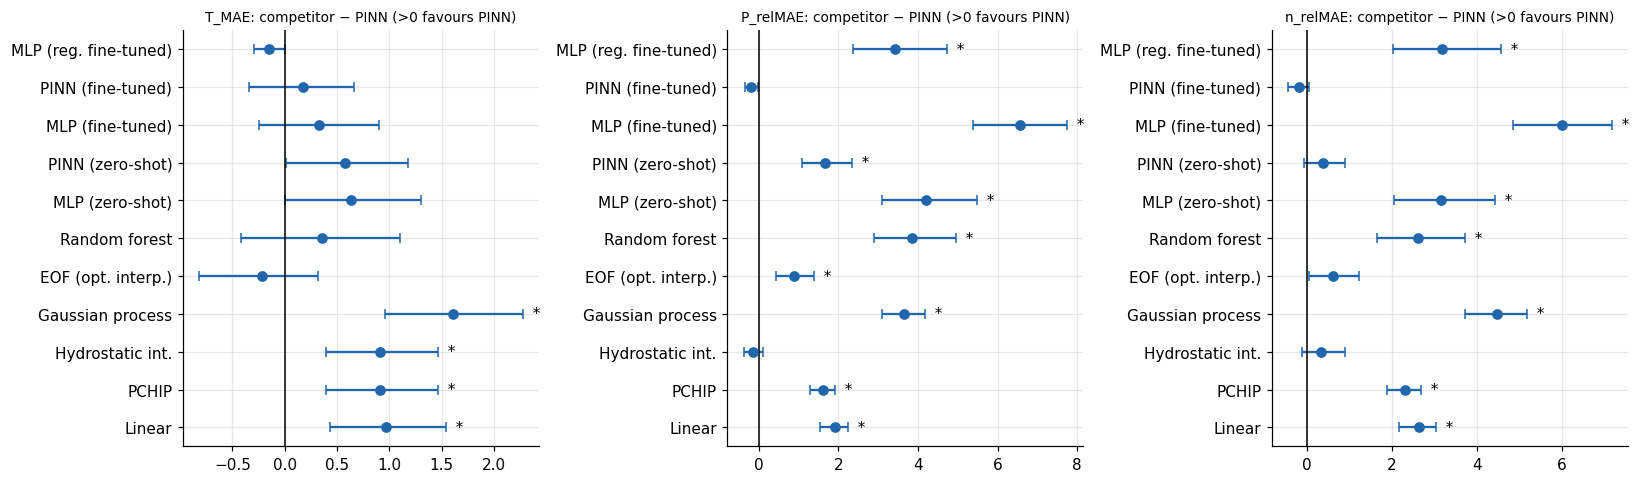
\includegraphics[width=\textwidth]{fig06_paired.png}
\caption{Paired difference between each competitor and \ours\ (competitor error minus \ours\ error) for temperature MAE, pressure error and density error, with 95\,\% bootstrap confidence intervals over profiles. Points to the right of zero favour \ours; asterisks mark Holm-corrected significance.}
\label{fig:paired}
\end{figure}

\subsection{Dependence on gap size and location (RQ2)}
\Cref{fig:gapsize} breaks down errors by gap size and location, and \cref{fig:examples} shows two example reconstructions.

\emph{Middle gaps (interpolation).} For small interior gaps the simple methods are hard to beat: with observed data on both sides, PCHIP and hydrostatic integration give temperature errors well below 1\,K at 2\,km, and hydrostatic integration gives the lowest pressure error at every gap size (about 0.005\,\% at 2\,km to 0.4\,\% at 20\,km). Here, \ours\ is significantly worse than hydrostatic integration for pressure ($\Delta=-0.57$\,\%, $p_\mathrm{Holm}=1.6\times10^{-7}$) and significantly worse than the regularised MLP for temperature ($\Delta=-0.24$\,K, $p_\mathrm{Holm}=0.037$). For temperature, interpolation remains as accurate as or more accurate than the learned methods at every middle-gap size.

\emph{Lower and upper gaps (extrapolation).} Here the picture reverses. Straight-line extrapolation and the GP grow rapidly worse with gap size, reaching about 8--10\,K temperature error and over 10\,\% pressure error at 20\,km. Methods that use other profiles stay roughly flat with gap size (about 2.5--4\,K at 20\,km). For pressure in upper gaps, \ours\ keeps errors around 1.5--2\,\% for all sizes, whereas data-only networks reach 5--16\,\%. In these extrapolation settings \ours\ is not significantly different from EOF, the regularised MLP, or hydrostatic integration for the tested comparisons.

\begin{figure}[p]
\centering
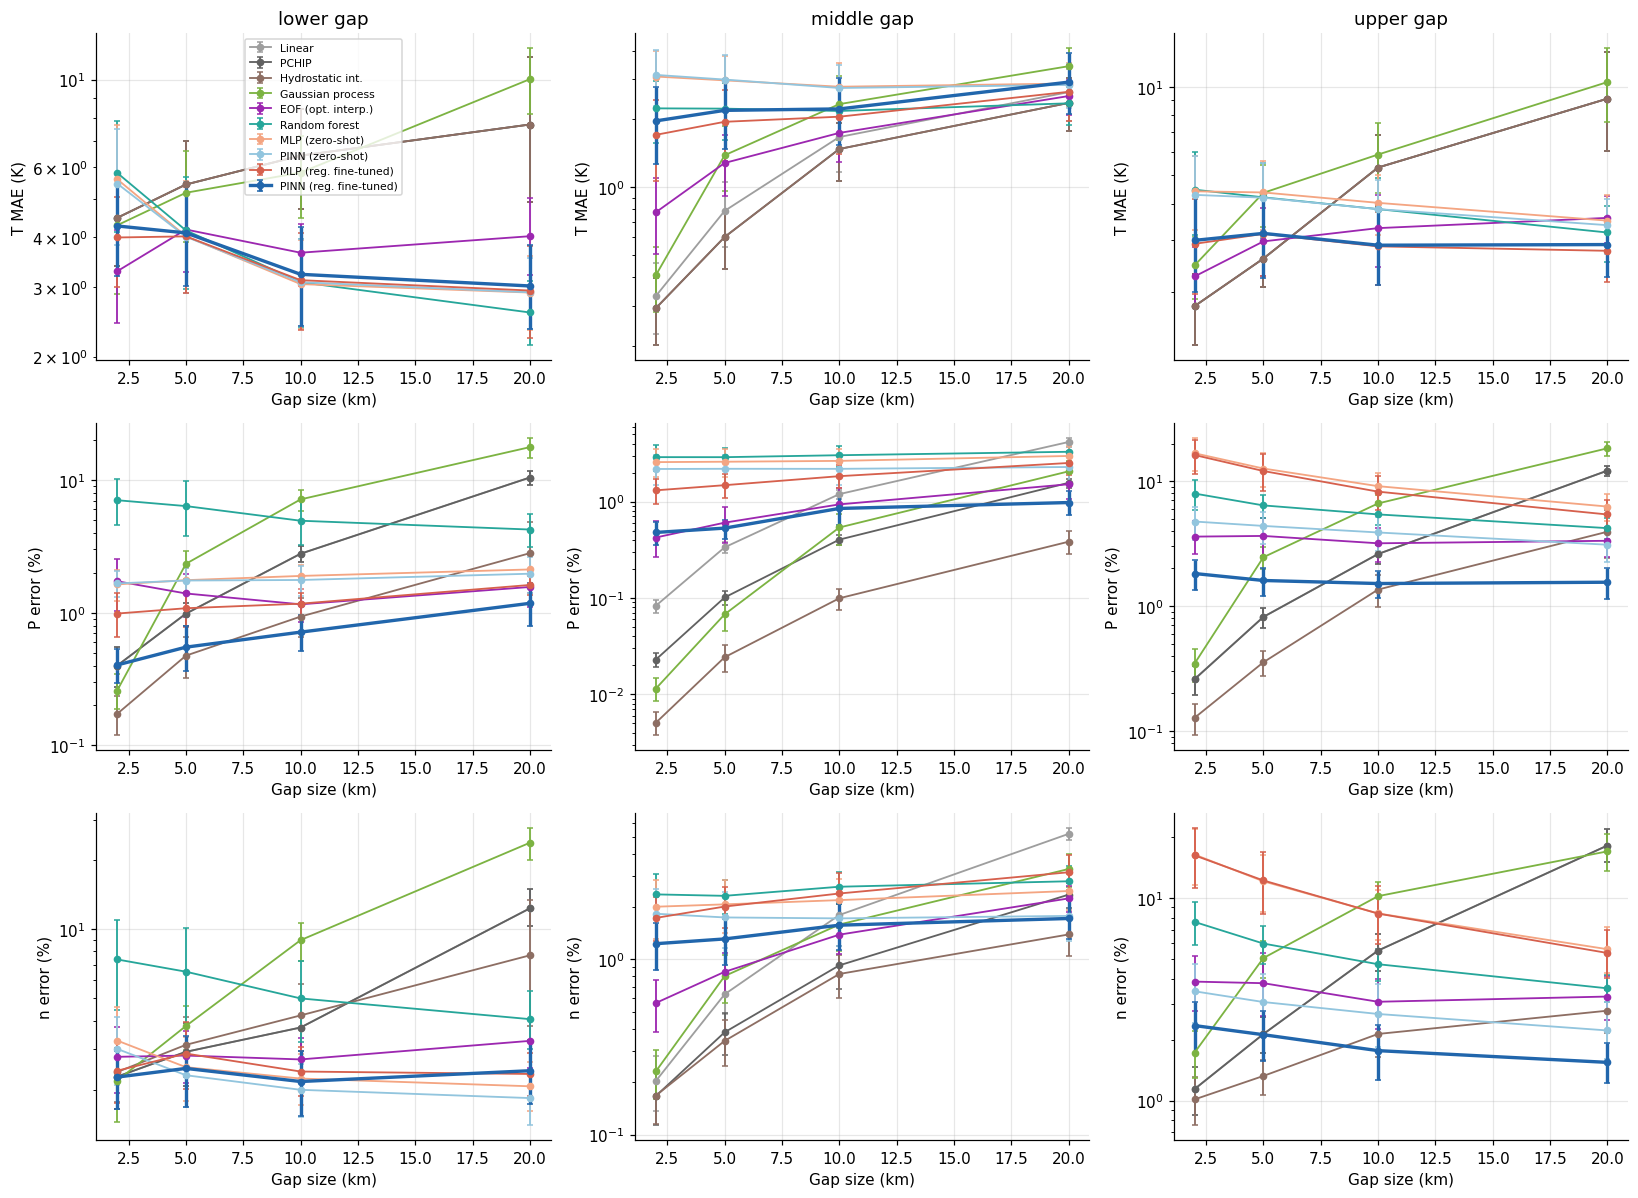
\includegraphics[width=\textwidth]{fig03_gap_size.png}
\caption{Error against gap size for lower (left), middle (centre) and upper (right) gaps: temperature MAE (top), pressure error (middle) and density error (bottom), on a logarithmic scale. Bars are 95\,\% bootstrap confidence intervals over profiles. \ours\ is the thick dark-blue line.}
\label{fig:gapsize}
\end{figure}

\begin{figure}[p]
\centering
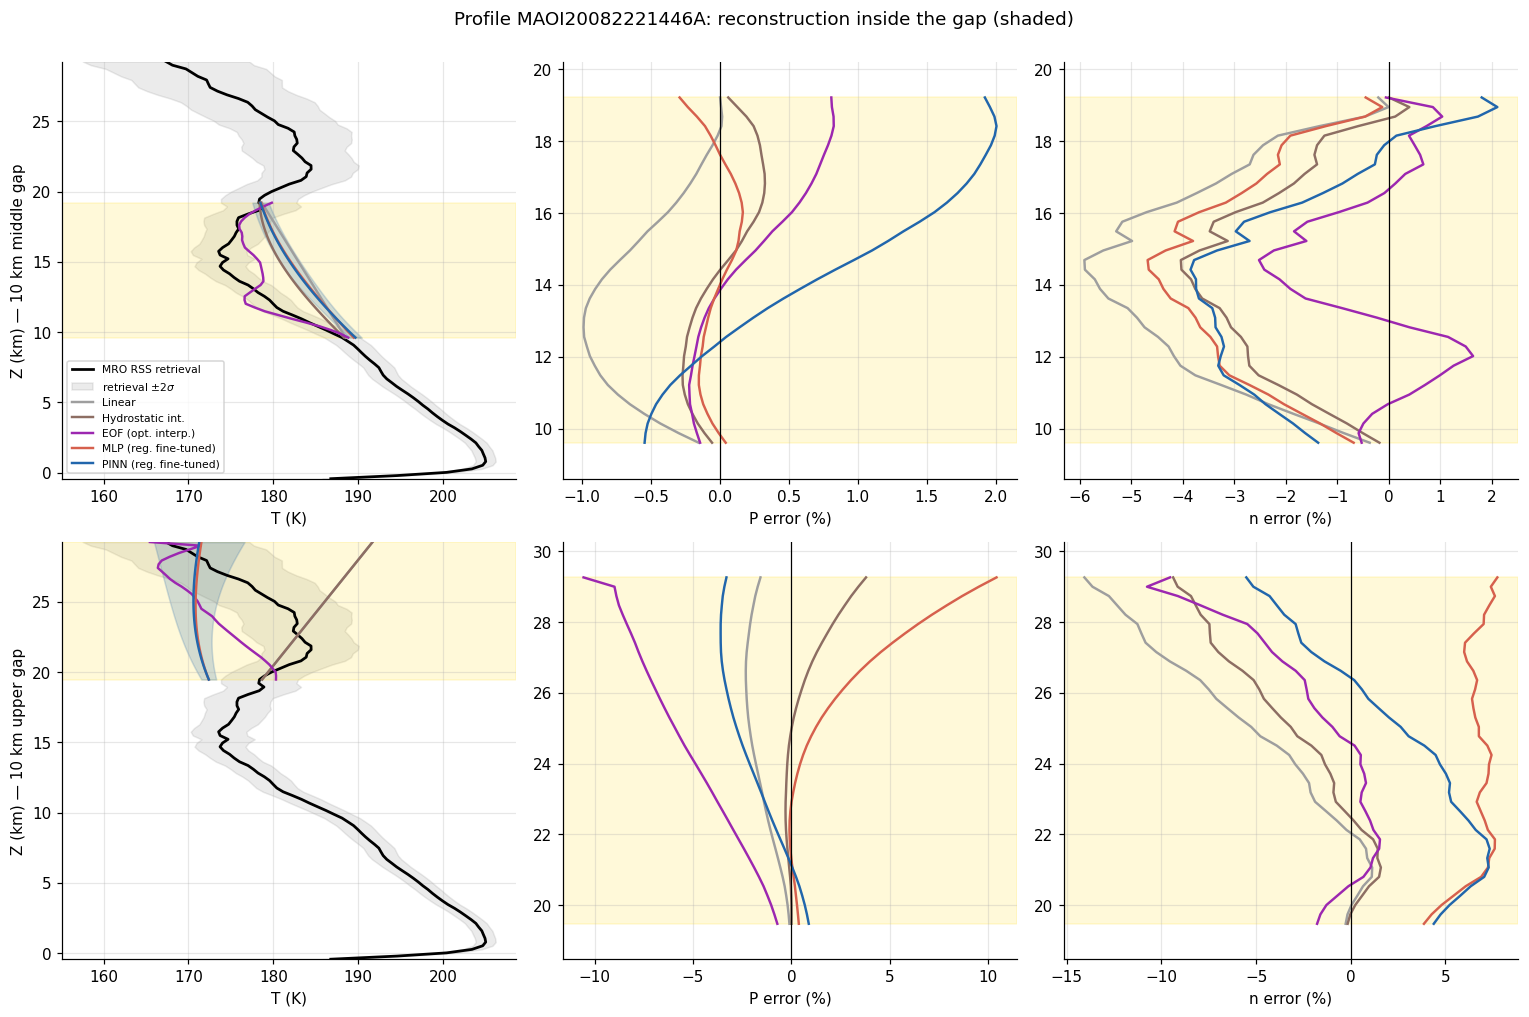
\includegraphics[width=\textwidth]{fig02_examples.png}
\caption{Example reconstructions for one test profile with a 10\,km middle gap (top row) and a 10\,km upper gap (bottom row). Left: temperature (black, reference with $\pm2\sigma$ band; shaded yellow, hidden interval; the blue band is the 95\,\% ensemble interval of \ours). Centre and right: pressure and density errors inside the gap.}
\label{fig:examples}
\end{figure}

\subsection{Physical consistency}
\Cref{fig:hydro} and the last column of \cref{tab:main} show the hydrostatic residual of each reconstruction. The physics term reduces the residual of the network by more than an order of magnitude: from 0.12 (regularised MLP) to 0.010 (\ours), and to 0.0031 for the plain fine-tuned PINN, which is within a factor of two of the reference floor (0.0016) and equal to that of exact hydrostatic integration. Methods that learn $T$ and $\ln P$ separately (EOF, random forest, MLPs) produce profiles that are noticeably inconsistent with hydrostatic balance, which is why their pressure and density errors are large even when their temperature is accurate.

\begin{figure}[t]
\centering
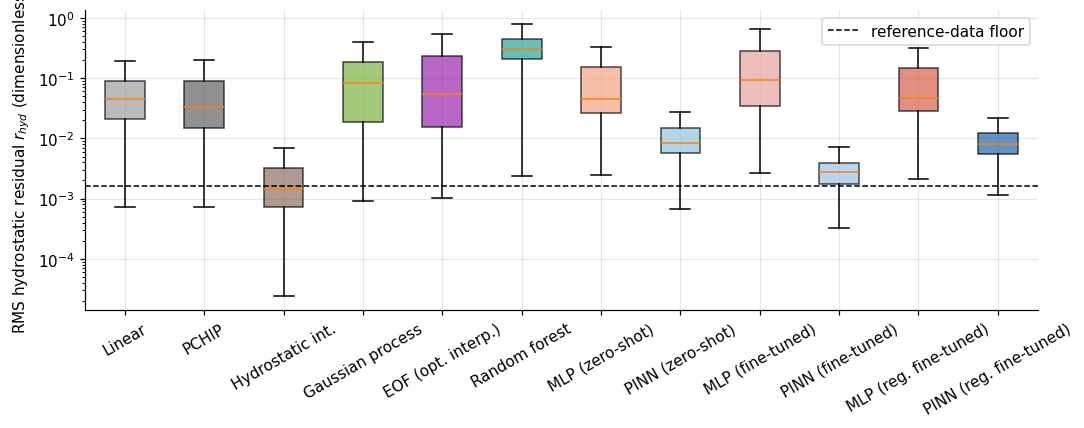
\includegraphics[width=\textwidth]{fig04_hydro_residual.png}
\caption{Distribution over test cases of the RMS hydrostatic residual of each reconstruction (logarithmic scale; boxes show quartiles). The dashed line is the floor of the reference data.}
\label{fig:hydro}
\end{figure}

\subsection{Uncertainty (RQ4)}
\Cref{tab:uq} and \cref{fig:calib} report the quality of the uncertainty estimates.

\emph{Raw intervals.} The EOF intervals are close to nominal (95\,\% intervals cover 96\,\% of temperatures). The GP and all neural ensembles are over-confident for temperature: their nominal 95\,\% intervals contain only 63--83\,\% of true values. For pressure, the PINN ensembles are close to nominal (\ours: 96\,\%), whereas data-only ensembles and the GP are over-confident.

\emph{After conformal calibration.} Using validation profiles to rescale the intervals brings all calibrated methods close to the target: 95\,\% intervals cover 92--98\,\% of temperatures and 94--98\,\% of $\ln P$ values on the unseen test profiles (\ours: 92\,\% and 94\,\%).

\emph{Ranking of errors.} Predicted uncertainty is positively but moderately correlated with actual error (Spearman $\rho$ 0.22--0.60 for temperature). EOF ($\rho=0.49$) and the plain fine-tuned ensembles ($\rho=0.54$--0.60) rank errors best; \ours\ ($\rho=0.31$) and the GP ($\rho=0.28$) less well.

\begin{table}[t]
\centering\small
\caption{Uncertainty quality on test profiles. Raw: empirical coverage of nominal 50/90/95\,\% Gaussian intervals. Conformal: coverage of 90/95\,\% intervals after split-conformal calibration on validation profiles (computed for four methods). $\rho$: Spearman correlation of predicted $\sigma$ with absolute error. Ideal coverage equals the nominal level.}\label{tab:uq}
\setlength{\tabcolsep}{3.5pt}
\begin{tabular}{l*{6}{c}*{4}{c}cc}
\toprule
& \multicolumn{6}{c}{Raw coverage} & \multicolumn{4}{c}{Conformal coverage} & \multicolumn{2}{c}{$\rho(\sigma,|e|)$}\\
\cmidrule(lr){2-7}\cmidrule(lr){8-11}\cmidrule(l){12-13}
Method & T50 & P50 & T90 & P90 & T95 & P95 & T90 & P90 & T95 & P95 & $T$ & $\ln P$\\
\midrule
EOF & 0.61 & 0.64 & 0.92 & 0.86 & 0.96 & 0.89 & 0.93 & 0.92 & 0.98 & 0.97 & 0.49 & 0.56\\
Gaussian process & 0.51 & 0.57 & 0.75 & 0.71 & 0.79 & 0.74 & 0.93 & 0.95 & 0.96 & 0.98 & 0.28 & 0.76\\
MLP (zero-shot) & 0.28 & 0.34 & 0.60 & 0.68 & 0.65 & 0.74 & -- & -- & -- & -- & 0.26 & 0.33\\
PINN (zero-shot) & 0.27 & 0.33 & 0.58 & 0.67 & 0.63 & 0.73 & -- & -- & -- & -- & 0.22 & 0.22\\
MLP (fine-tuned) & 0.49 & 0.43 & 0.78 & 0.76 & 0.83 & 0.81 & -- & -- & -- & -- & 0.60 & 0.67\\
PINN (fine-tuned) & 0.46 & 0.77 & 0.73 & 0.90 & 0.77 & 0.92 & -- & -- & -- & -- & 0.54 & 0.64\\
MLP (reg.\ ft) & 0.40 & 0.53 & 0.71 & 0.82 & 0.76 & 0.88 & 0.85 & 0.88 & 0.91 & 0.94 & 0.37 & 0.38\\
\textbf{\ours} & 0.38 & 0.66 & 0.67 & 0.94 & 0.73 & 0.96 & 0.87 & 0.89 & 0.92 & 0.94 & 0.31 & 0.40\\
\bottomrule
\end{tabular}
\end{table}

\begin{figure}[t]
\centering
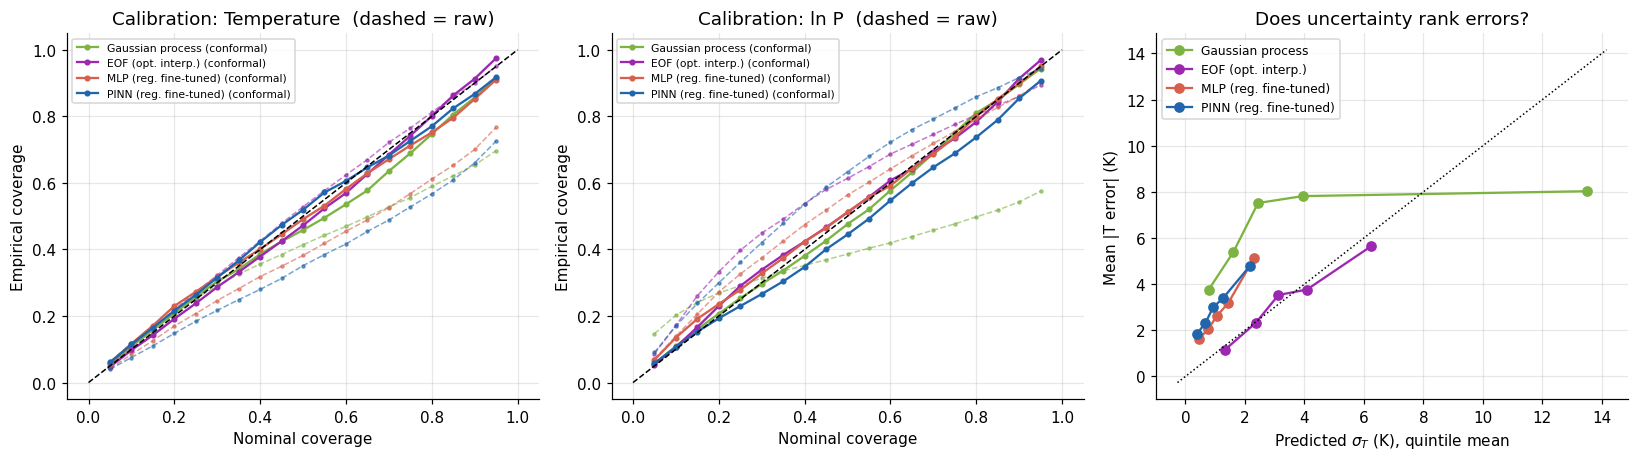
\includegraphics[width=\textwidth]{fig05_calibration.png}
\caption{Calibration of predictive intervals. Left and centre: empirical against nominal coverage for temperature and $\ln P$ (dashed: raw intervals; solid: after conformal calibration; the black diagonal is perfect calibration). Right: mean absolute temperature error against predicted $\sigma_T$, grouped into quintiles; a well-ranked uncertainty follows an increasing line.}
\label{fig:calib}
\end{figure}

\subsection{Robustness to noisy inputs (RQ3)}
\Cref{tab:noise} and \cref{fig:noise} show what happens when noise is added to the observed levels (10\,km middle gaps). Without added noise, simple interpolation is most accurate for temperature (PCHIP 1.47\,K). As noise grows, methods that follow the observed points closely degrade fastest: at five times the retrieval uncertainty PCHIP and hydrostatic integration reach 5.31\,K and EOF 4.48\,K. The neural networks, which are anchored to a learned prior and regularised toward it, barely change: \ours\ goes from 2.36 to 2.82\,K and the regularised MLP from 1.99 to 2.50\,K. For pressure (\cref{fig:noise}, right), \ours\ remains the most accurate method under noise (roughly 1\,\%), whereas hydrostatic integration, which is best without noise, degrades by more than an order of magnitude because it is anchored to the (now noisy) pressures at the gap edges.

\begin{table}[t]
\centering\small
\caption{Temperature MAE (K) for 10\,km middle gaps when Gaussian noise of $k$ times the retrieval uncertainty is added to the observed levels (27 test profiles).}\label{tab:noise}
\begin{tabular}{lccc}
\toprule
Method & $k=0$ & $k=2$ & $k=5$\\
\midrule
Linear & 1.66 & 2.45 & 4.29\\
PCHIP & 1.47 & 3.19 & 5.31\\
Hydrostatic int. & 1.47 & 3.19 & 5.31\\
Gaussian process & 2.32 & 2.87 & 3.36\\
EOF (opt.\ interp.) & 1.73 & 2.58 & 4.48\\
MLP (reg.\ fine-tuned) & 1.99 & 2.17 & 2.50\\
\textbf{\ours} & 2.36 & 2.40 & 2.82\\
\bottomrule
\end{tabular}
\end{table}

\begin{figure}[t]
\centering
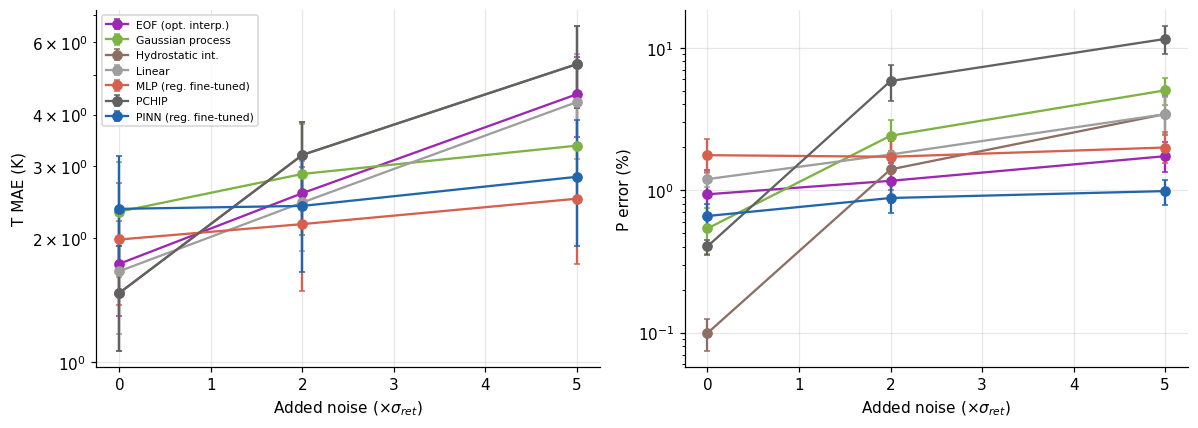
\includegraphics[width=0.9\textwidth]{fig07_noise.png}
\caption{Effect of added observation noise (in multiples of the retrieval uncertainty) on temperature MAE (left) and pressure error (right) for 10\,km middle gaps.}
\label{fig:noise}
\end{figure}

\subsection{Sensitivity to the physics weight (RQ3)}
\Cref{tab:lambda} and \cref{fig:lambda} vary the physics weight $\lambda$ used during (plain) fine-tuning. Turning physics off ($\lambda=0$) gives the worst pressure and density, especially for upper gaps (7.0\,\% pressure error), and a large hydrostatic residual. Any $\lambda$ between 0.1 and 10 gives pressure errors of 0.3--0.6\,\% (middle) and 1.1--1.4\,\% (upper), and residuals close to the floor. Very large weights ($\lambda=100$) over-constrain the network: the physics term dominates the data term, and temperature errors grow sharply (to 7.5\,K for upper gaps). Temperature error increases slowly and steadily with $\lambda$, which confirms that the physics constraint does not by itself improve temperature. The method is thus insensitive to $\lambda$ over two orders of magnitude, and the validation-selected value ($\lambda=0.1$) lies in the flat optimum.

\begin{table}[t]
\centering\small
\caption{Sensitivity of the plain fine-tuned PINN to the physics weight $\lambda$ (27 test profiles, one seed; 10\,km gaps). Hydro.: RMS hydrostatic residual (floor 0.0016).}\label{tab:lambda}
\begin{tabular}{l*{4}{c}@{\hspace{12pt}}*{4}{c}}
\toprule
& \multicolumn{4}{c}{Middle gap} & \multicolumn{4}{c}{Upper gap}\\
\cmidrule(r){2-5}\cmidrule(l){6-9}
$\lambda$ & T (K) & P (\%) & $n$ (\%) & Hydro. & T (K) & P (\%) & $n$ (\%) & Hydro.\\
\midrule
0 & 1.41 & 0.97 & 1.45 & 0.0230 & 3.65 & 7.04 & 7.95 & 0.1505\\
0.01 & 1.45 & 0.71 & 1.08 & 0.0127 & 3.74 & 1.61 & 1.87 & 0.0236\\
0.1 & 1.42 & 0.32 & 0.71 & 0.0045 & 3.79 & 1.12 & 1.43 & 0.0069\\
1 & 1.48 & 0.40 & 0.73 & 0.0029 & 3.98 & 1.12 & 1.52 & 0.0042\\
10 & 1.80 & 0.60 & 0.77 & 0.0041 & 4.41 & 1.38 & 1.64 & 0.0045\\
100 & 2.47 & 0.88 & 1.02 & 0.0132 & 7.53 & 3.05 & 2.34 & 0.0130\\
\bottomrule
\end{tabular}
\end{table}

\begin{figure}[t]
\centering
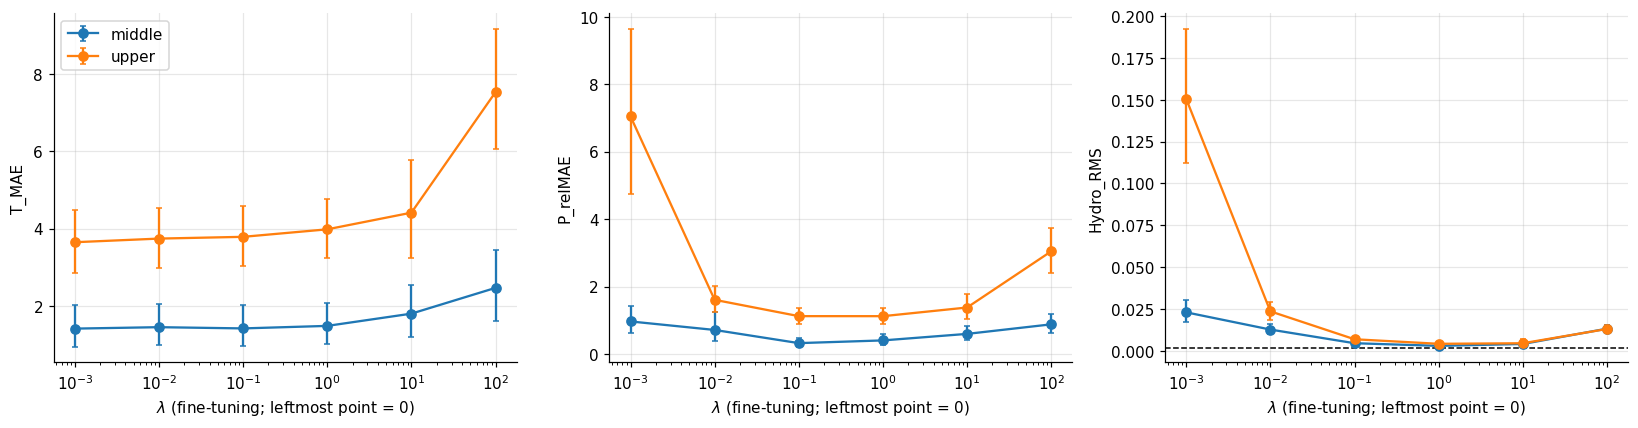
\includegraphics[width=\textwidth]{fig08_lambda.png}
\caption{Sensitivity to the physics weight $\lambda$ during fine-tuning: temperature MAE, pressure error and hydrostatic residual for 10\,km middle and upper gaps. The leftmost point is $\lambda=0$; the dashed line is the reference floor.}
\label{fig:lambda}
\end{figure}

\subsection{Transfer to an unseen Mars year (RQ5)}\label{sec:holdout}
\Cref{tab:holdout} and \cref{fig:holdout} show temperature errors when one Mars year is held out entirely. Holding out MY\,29 is by far the hardest case: it is the only year covering low latitudes and late northern summer (\cref{fig:data}a), so the training data contain nothing similar. Zero-shot networks fail badly there (13.7\,K for the MLP and 24.5\,K for the PINN), showing that a learned climatology cannot be trusted outside the conditions it was trained on. Fine-tuning on the observed part of the profile rescues the networks: \ours\ has the lowest temperature error for MY\,29 (6.46\,K) and is within 0.3\,K of the best method for the other two years. Hydrostatic integration, which uses no other profiles, is equally competitive, and EOF does best for MY\,31.

\begin{table}[t]
\centering\small
\caption{Temperature MAE (K) when the indicated Mars year is held out from training (10\,km middle and upper gaps). Best per column in bold.}\label{tab:holdout}
\begin{tabular}{lccc}
\toprule
Method & MY 29 held out & MY 30 held out & MY 31 held out\\
\midrule
Hydrostatic int. & 6.52 & \textbf{2.73} & 2.17\\
Gaussian process & 7.26 & 4.06 & 3.65\\
EOF (opt.\ interp.) & 7.18 & 3.05 & \textbf{1.88}\\
Random forest & 8.79 & 5.57 & 2.61\\
MLP (zero-shot) & 13.73 & 4.70 & 4.61\\
PINN (zero-shot) & 24.50 & 5.15 & 5.71\\
MLP (reg.\ fine-tuned) & 6.71 & 3.05 & 2.34\\
\textbf{\ours} & \textbf{6.46} & 3.02 & 2.15\\
\bottomrule
\end{tabular}
\end{table}

\begin{figure}[t]
\centering
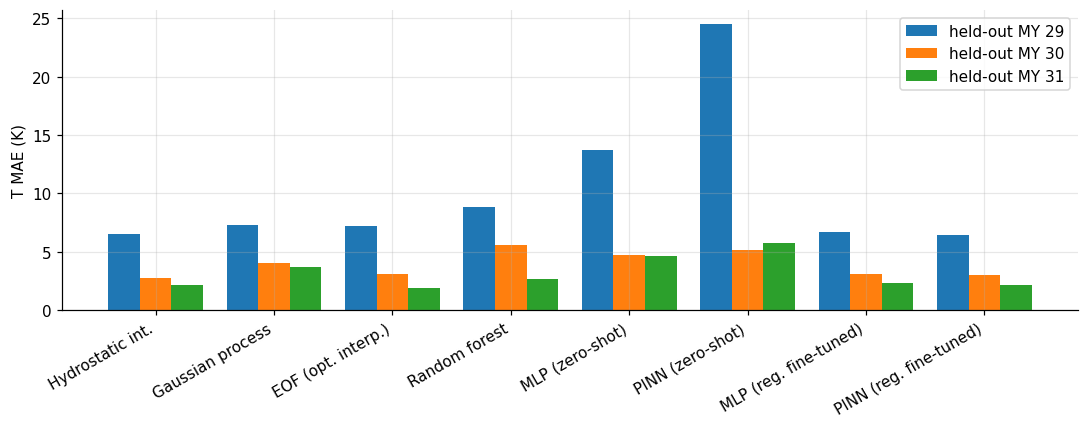
\includegraphics[width=0.9\textwidth]{fig09_holdout.png}
\caption{Temperature MAE for each Mars-year hold-out experiment.}
\label{fig:holdout}
\end{figure}

\subsection{Training behaviour}
\Cref{fig:training} shows that pre-training converges smoothly. The physics loss of the PINN falls by more than two orders of magnitude to about $10^{-4}$. The validation data loss of the PINN is similar to or slightly lower than that of the MLP late in training, while several MLP runs begin to over-fit after about 1000 epochs (the checkpoint with the lowest validation loss is kept, so this does not affect the selected models). The physics term thus acts partly as a regulariser.

\begin{figure}[t]
\centering
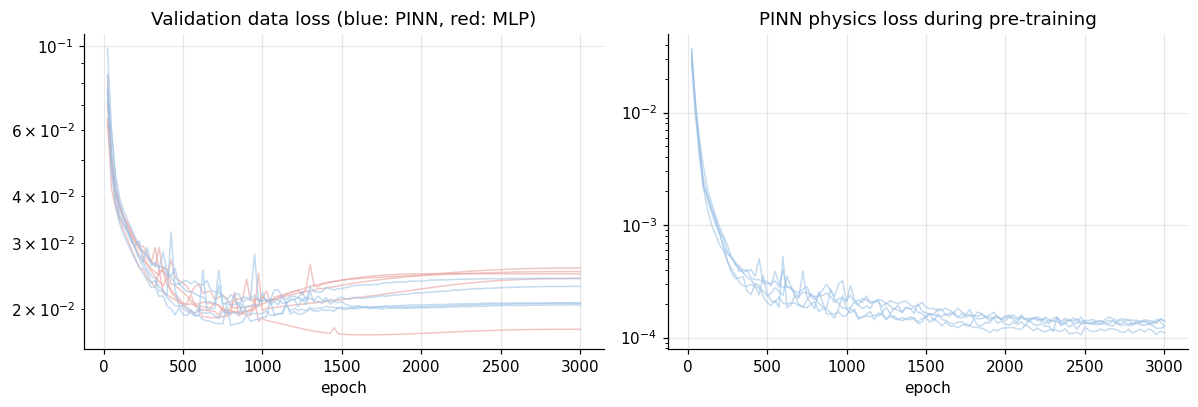
\includegraphics[width=0.9\textwidth]{fig10_training.png}
\caption{Pre-training curves for the five seeds of each family. Left: validation data loss (blue: PINN, red: MLP). Right: physics loss of the PINN.}
\label{fig:training}
\end{figure}

% ==================================================================
\section{Discussion}\label{sec:discussion}
% ==================================================================

\subsection{What the physics buys --- and what it does not}
The clearest result of this study is that hydrostatic physics mainly improves \emph{pressure and density}, not temperature. This is expected from \cref{eq:hydroZ}: hydrostatic balance determines how $\ln P$ changes with height \emph{given} $T$, so a network that obeys it automatically turns its temperature estimate into a consistent pressure profile. A data-only network, in contrast, learns $T$ and $\ln P$ as two separate outputs; small inconsistencies between them accumulate over the height of a gap and produce pressure errors of several percent. The same is true for EOF, random forest and the GP.

Temperature inside a gap, on the other hand, is set by the learned cross-profile prior and the observed data at the edges. Physics cannot add information here, and indeed temperature error rises slightly as the physics weight grows (\cref{tab:lambda}). EOF optimal interpolation, which is essentially an optimal linear statistical prior, is therefore an appropriate and strong benchmark for temperature, and the PINN does not beat it.

\begin{plainbox}
The physics rule is like a recipe that tells you how much the pressure must change for a given temperature. If you have the temperature right, the recipe gives you the right pressure. But the recipe does not tell you what the temperature is --- for that you need either the measurements nearby or experience from many similar profiles.
\end{plainbox}

\subsection{Interpolation versus extrapolation}
When data exist on both sides of a small gap, simple interpolation of temperature followed by exact hydrostatic integration is hard to beat, cheap, and transparent. The advantages of learned methods appear for gaps at the ends of a profile and for large gaps, where there is nothing on one side to interpolate from, and when the observed data are noisy.

\subsection{Practical recommendations}
\begin{itemize}[leftmargin=*]
\item For \textbf{small interior gaps} with good data: interpolate temperature (PCHIP) and integrate hydrostatic balance for pressure.
\item For \textbf{temperature} in large or end gaps: EOF optimal interpolation or a regularised fine-tuned network; both are comparably accurate, and EOF gives the best-calibrated uncertainties without extra calibration.
\item For \textbf{pressure and density} in large or end gaps, or when the observed data are \textbf{noisy}: a physics-informed network fine-tuned with regularisation (\ours) is the most consistent choice.
\item Always pair neural ensembles with a \textbf{calibration step} (e.g.\ split-conformal prediction) before using their uncertainty ranges.
\item Do not use a pre-trained network \textbf{zero-shot} outside the seasons and latitudes it was trained on.
\end{itemize}
A natural combination, which we leave for future work, would use an EOF-type prior for temperature and enforce hydrostatic balance for pressure inside the same model.

\subsection{Limitations}
\begin{enumerate}[leftmargin=*]
\item \textbf{Scope of the data.} All 184 profiles are pre-dawn ingress occultations in northern spring and summer of the low-dust season, at latitudes of about $13^\circ$S--$69^\circ$N. Conclusions may not hold for dusty seasons, daytime conditions or southern latitudes.
\item \textbf{The reference is a retrieval, not ground truth.} It carries its own uncertainty and was produced using hydrostatic balance and the ideal-gas law. Physical-consistency results measure agreement with the retrieval physics.
\item \textbf{Physics constrains pressure given temperature, not temperature itself.} Any temperature differences between the PINN and the data-only network should be interpreted with this in mind.
\item \textbf{Synthetic gaps.} Gaps were imposed on complete profiles; real data losses may have different structure, e.g.\ partially degraded rather than entirely missing levels.
\item \textbf{Trimmed top.} Levels with $\sigma_T>5$\,K were removed, so results do not cover the upper initialisation zone, where reconstruction would arguably be most useful.
\item \textbf{Sample size.} With 28 test profiles, moderate differences (e.g.\ 0.2\,K in temperature) cannot be resolved statistically; non-significant results should be read as ``no evidence of a difference'', not as evidence of equivalence.
\item \textbf{Confounding of year and season.} In the hold-out experiment the effects of an unseen year and an unseen season cannot be separated.
\end{enumerate}

% ==================================================================
\section{Conclusions}\label{sec:conclusion}
% ==================================================================
We built a careful benchmark for reconstructing missing intervals in Martian radio-occultation profiles and compared a physics-informed neural network with eleven alternatives. Enforcing the ideal-gas law exactly and hydrostatic balance through a dimensionless residual in geopotential height makes the network's pressure and density about four times more accurate than those of an otherwise identical data-only network (1.0\,\% versus 4.4\,\% for pressure) and keeps its profiles close to exact hydrostatic balance. The physics also makes the network robust to noisy inputs and, after conformal calibration, its uncertainty ranges reach near-nominal coverage. For temperature, however, the physics adds no information: EOF optimal interpolation and a regularised data-only network are equally accurate, and for small interior gaps simple interpolation with hydrostatic integration remains the best and cheapest choice. Physics-informed learning is therefore most valuable here as a way to keep reconstructed profiles thermodynamically consistent, particularly for large gaps at the ends of a profile and for noisy data.

% ------------------------------------------------------------------
\section*{Code and data availability}
The MRO RSS data are publicly available from NASA's Planetary Data System as product \texttt{MRO-M-RSS-5-TPS-V1.0} \citep{hinsonPDS}. The complete experiment --- data audit, splits, all methods, experiments, statistics, figures and tables --- is contained in a single Jupyter notebook that writes every number reported here; it will be made available by the authors upon publication. All random seeds, splits and selected hyper-parameters are saved by the notebook (\cref{app:hyper}).

\section*{Author contributions}
S.D.\ and K.A.\ conceived the study. K.A.\ designed and implemented the experiments. Both authors analysed the results and wrote the manuscript.

\section*{Acknowledgements}
We thank D.\,P.\ Hinson and the MRO Radio Science team for producing and archiving the temperature--pressure profiles used in this work.

\section*{Competing interests}
The authors declare no competing interests.

% ------------------------------------------------------------------
\begin{thebibliography}{99}
\setlength{\itemsep}{2pt}\small

\bibitem[Angelopoulos and Bates(2023)]{angelopoulos2023}
Angelopoulos, A.\,N., \& Bates, S. (2023). Conformal prediction: A gentle introduction. \emph{Foundations and Trends in Machine Learning}, 16(4), 494--591.

\bibitem[Beckers and Rixen(2003)]{beckers2003}
Beckers, J.-M., \& Rixen, M. (2003). EOF calculations and data filling from incomplete oceanographic datasets. \emph{Journal of Atmospheric and Oceanic Technology}, 20(12), 1839--1856.

\bibitem[Breiman(2001)]{breiman2001}
Breiman, L. (2001). Random forests. \emph{Machine Learning}, 45(1), 5--32.

\bibitem[Clancy et~al.(2000)]{clancy2000}
Clancy, R.\,T., Sandor, B.\,J., Wolff, M.\,J., Christensen, P.\,R., Smith, M.\,D., Pearl, J.\,C., Conrath, B.\,J., \& Wilson, R.\,J. (2000). An intercomparison of ground-based millimeter, MGS TES, and Viking atmospheric temperature measurements: Seasonal and interannual variability of temperatures and dust loading in the global Mars atmosphere. \emph{Journal of Geophysical Research: Planets}, 105(E4), 9553--9571.

\bibitem[Efron(1979)]{efron1979}
Efron, B. (1979). Bootstrap methods: Another look at the jackknife. \emph{The Annals of Statistics}, 7(1), 1--26.

\bibitem[Fjeldbo et~al.(1971)]{fjeldbo1971}
Fjeldbo, G., Kliore, A.\,J., \& Eshleman, V.\,R. (1971). The neutral atmosphere of Venus as studied with the Mariner V radio occultation experiments. \emph{The Astronomical Journal}, 76, 123--140.

\bibitem[Fritsch and Carlson(1980)]{fritsch1980}
Fritsch, F.\,N., \& Carlson, R.\,E. (1980). Monotone piecewise cubic interpolation. \emph{SIAM Journal on Numerical Analysis}, 17(2), 238--246.

\bibitem[Hinson et~al.(1999)]{hinson1999}
Hinson, D.\,P., Simpson, R.\,A., Twicken, J.\,D., Tyler, G.\,L., \& Flasar, F.\,M. (1999). Initial results from radio occultation measurements with Mars Global Surveyor. \emph{Journal of Geophysical Research: Planets}, 104(E11), 26997--27012.

\bibitem[Hinson(PDS)]{hinsonPDS}
Hinson, D.\,P. MRO Radio Science Subsystem temperature--pressure profiles, \texttt{MRO-M-RSS-5-TPS-V1.0}. NASA Planetary Data System, Atmospheres Node.

\bibitem[Holm(1979)]{holm1979}
Holm, S. (1979). A simple sequentially rejective multiple test procedure. \emph{Scandinavian Journal of Statistics}, 6(2), 65--70.

\bibitem[Karniadakis et~al.(2021)]{karniadakis2021}
Karniadakis, G.\,E., Kevrekidis, I.\,G., Lu, L., Perdikaris, P., Wang, S., \& Yang, L. (2021). Physics-informed machine learning. \emph{Nature Reviews Physics}, 3(6), 422--440.

\bibitem[Kingma and Ba(2015)]{kingma2015}
Kingma, D.\,P., \& Ba, J. (2015). Adam: A method for stochastic optimization. In \emph{International Conference on Learning Representations (ICLR)}.

\bibitem[Kursinski et~al.(1997)]{kursinski1997}
Kursinski, E.\,R., Hajj, G.\,A., Schofield, J.\,T., Linfield, R.\,P., \& Hardy, K.\,R. (1997). Observing Earth's atmosphere with radio occultation measurements using the Global Positioning System. \emph{Journal of Geophysical Research: Atmospheres}, 102(D19), 23429--23465.

\bibitem[Lakshminarayanan et~al.(2017)]{lakshminarayanan2017}
Lakshminarayanan, B., Pritzel, A., \& Blundell, C. (2017). Simple and scalable predictive uncertainty estimation using deep ensembles. In \emph{Advances in Neural Information Processing Systems 30}, 6402--6413.

\bibitem[Li et~al.(2018)]{li2018l2sp}
Li, X., Grandvalet, Y., \& Davoine, F. (2018). Explicit inductive bias for transfer learning with convolutional networks. In \emph{Proceedings of the 35th International Conference on Machine Learning (ICML)}, 2825--2834.

\bibitem[Paszke et~al.(2019)]{paszke2019}
Paszke, A., et~al. (2019). PyTorch: An imperative style, high-performance deep learning library. In \emph{Advances in Neural Information Processing Systems 32}, 8024--8035.

\bibitem[Pedregosa et~al.(2011)]{pedregosa2011}
Pedregosa, F., et~al. (2011). Scikit-learn: Machine learning in Python. \emph{Journal of Machine Learning Research}, 12, 2825--2830.

\bibitem[Raissi et~al.(2019)]{raissi2019}
Raissi, M., Perdikaris, P., \& Karniadakis, G.\,E. (2019). Physics-informed neural networks: A deep learning framework for solving forward and inverse problems involving nonlinear partial differential equations. \emph{Journal of Computational Physics}, 378, 686--707.

\bibitem[Rasmussen and Williams(2006)]{rasmussen2006}
Rasmussen, C.\,E., \& Williams, C.\,K.\,I. (2006). \emph{Gaussian Processes for Machine Learning}. MIT Press.

\bibitem[Vovk et~al.(2005)]{vovk2005}
Vovk, V., Gammerman, A., \& Shafer, G. (2005). \emph{Algorithmic Learning in a Random World}. Springer.

\bibitem[Wilcoxon(1945)]{wilcoxon1945}
Wilcoxon, F. (1945). Individual comparisons by ranking methods. \emph{Biometrics Bulletin}, 1(6), 80--83.

\bibitem[Zurek and Smrekar(2007)]{zurek2007}
Zurek, R.\,W., \& Smrekar, S.\,E. (2007). An overview of the Mars Reconnaissance Orbiter (MRO) science mission. \emph{Journal of Geophysical Research: Planets}, 112(E5), E05S01.

\end{thebibliography}

% ==================================================================
\appendix
\clearpage
\section{Glossary}\label{app:glossary}
\begin{description}[leftmargin=0.4cm,style=nextline,itemsep=2pt]
\item[Bootstrap confidence interval] A range for a quantity obtained by repeatedly re-sampling the test profiles with replacement and recomputing the quantity; the middle 95\,\% of these values forms the interval.
\item[Calibration] Agreement between stated and actual confidence: a calibrated 90\,\% interval contains the true value 90\,\% of the time.
\item[Collocation point] A location (coordinates only) where the physics equation is checked during training, even if no measurement exists there.
\item[Conformal prediction] A method that rescales error bars using a separate calibration set so that they reach a desired coverage.
\item[Deep ensemble] Several neural networks trained from different random starting points; their spread estimates uncertainty.
\item[EOF (empirical orthogonal function)] One of the dominant patterns of variation in a collection of profiles, obtained by principal component analysis.
\item[Extrapolation / interpolation] Estimating values outside / between the range of available data.
\item[Fine-tuning] Briefly continuing to train a pre-trained network on new data (here: the observed part of one profile).
\item[Geopotential height] A height coordinate based on gravitational potential energy, in which hydrostatic balance takes its simplest exact form.
\item[Holm correction] A procedure that adjusts $p$-values when many tests are made, to limit false discoveries.
\item[Hydrostatic balance] The condition that the pressure at any level supports the weight of the air above it.
\item[Ideal-gas law] $P=n\kB T$: the relation between pressure, number density and temperature of a dilute gas.
\item[L2-SP] A penalty that keeps fine-tuned network weights close to their pre-trained values.
\item[MAE] Mean absolute error: the average size of the errors, ignoring sign.
\item[Mars year (MY)] One orbit of Mars around the Sun (687 Earth days), numbered from 11 April 1955.
\item[Number density] Number of molecules per unit volume.
\item[PINN] Physics-informed neural network: a neural network trained to match data and satisfy physical equations.
\item[Radio occultation] Measuring an atmosphere by observing how it bends a radio signal passing through it.
\item[Scale height] The height over which pressure falls by a factor $e\approx2.718$; about 10\,km on Mars.
\item[Solar longitude $L_s$] The season on Mars, measured as the angle of Mars around its orbit from the northern spring equinox.
\item[Wilcoxon signed-rank test] A test of whether paired differences are systematically positive or negative, without assuming a normal distribution.
\item[Zero-shot] Using a trained model on a new case without adapting it to that case.
\end{description}

\section{Hyper-parameters and settings}\label{app:hyper}
\begin{table}[h]
\centering\small
\caption{Complete settings of the experiment.}\label{tab:hyper}
\begin{tabular}{lp{8.2cm}}
\toprule
Setting & Value\\
\midrule
Quality control & drop levels with $\sigma_T>5$\,K; keep profiles with strictly increasing $Z$ and $\ge40$ levels\\
Split & 70/15/15\,\% of profiles, stratified by Mars year, seed 2024\\
Gaps & 2, 5, 10, 20\,km; lower/middle/upper; $\ge5$\,km observed; $\ge3$ hidden and $\ge5$ observed levels\\
Constants & $g_0=3.71$\,m\,s$^{-2}$; $\Tref=200$\,K; $m=43.485$\,g\,mol$^{-1}$; $\Href=10.31$\,km\\
Network & MLP, 4 hidden layers $\times$ 64 units, tanh, Xavier-normal init., 13\,058 parameters\\
Inputs / outputs & $(Z,\varphi,\sin\lambda,\cos\lambda,\sin L_s,\cos L_s)$ / $(T,\ln P)$; $n=P/(\kB T)$\\
Data weights & $1/\max(\sigma,\sigma_\mathrm{floor})^2$; floors 0.5\,K and 0.003 in $\ln P$\\
Pre-training & Adam, lr $2\times10^{-3}$ cosine to $10^{-5}$, 3000 epochs, full batch, grad.\ clip 1; $\lambda=1$ (PINN); 200 collocation pts/profile, 2048 per epoch; model selection on validation data loss every 25 epochs\\
Fine-tuning & Adam, lr $5\times10^{-4}$, 400 steps; 64 collocation pts in gap + 32 along profile\\
Regularised FT (selected) & MLP: $\alpha=1$, no early stopping; PINN: $\lambda=0.1$, $\alpha=1$, no early stopping\\
Early stopping (when used) & hold out every 2nd level within 3\,km of gap; check every 25 steps\\
Ensemble & 5 seeds (0--4); 3 seeds in E2 and E4; 1 seed in E3 and tuning\\
GP & constant $\times$ RBF ($\ell\in[0.3,50]$\,km) + white noise; linear mean; 2 restarts\\
EOF & 0.5\,km grid, coverage $\ge20$\,\%, 99\,\% variance, $\le15$ modes (15 for $T$, 10 for $\ln P$)\\
Random forest & 300 trees, min.\ 3 samples per leaf\\
Extrapolation (interpolators) & linear fit to nearest 3\,km of observed data\\
Statistics & 5000 bootstrap resamples; Wilcoxon signed-rank; Holm correction; $\alpha=0.05$\\
\bottomrule
\end{tabular}
\end{table}

\section{Density comparison}\label{app:density}
\begin{table}[h]
\centering\small
\caption{Paired comparison of number-density error (\%) between each competitor and \ours\ (format as in \cref{tab:sig}).}\label{tab:sig_n}
\begin{tabular}{lrrrr}
\toprule
Competitor & $\Delta$ [95\,\% CI] & Impr.\ (\%) & Better & $p_\mathrm{Holm}$\\
\midrule
EOF (opt.\ interp.) & 0.60 [0.03, 1.21] & 23.9 & 0.71 & 0.23\\
Gaussian process$^\star$ & 4.47 [3.72, 5.19] & 69.9 & 0.96 & $1.6\times10^{-7}$\\
Hydrostatic int. & 0.33 [$-0.11$, 0.89] & 14.7 & 0.57 & 0.43\\
Linear$^\star$ & 2.63 [2.17, 3.03] & 57.8 & 0.96 & $4.7\times10^{-7}$\\
MLP (fine-tuned)$^\star$ & 6.02 [4.86, 7.17] & 75.8 & 0.96 & $1.6\times10^{-7}$\\
MLP (reg.\ fine-tuned)$^\star$ & 3.18 [2.01, 4.57] & 62.3 & 0.89 & $4\times10^{-5}$\\
MLP (zero-shot)$^\star$ & 3.16 [2.04, 4.42] & 62.2 & 0.86 & $5.5\times10^{-5}$\\
PCHIP$^\star$ & 2.31 [1.87, 2.69] & 54.6 & 0.96 & $6\times10^{-7}$\\
PINN (fine-tuned) & $-0.20$ [$-0.45$, 0.04] & $-11.5$ & 0.50 & 0.43\\
PINN (zero-shot) & 0.38 [$-0.07$, 0.88] & 16.4 & 0.64 & 0.43\\
Random forest$^\star$ & 2.61 [1.65, 3.72] & 57.7 & 0.86 & $4.8\times10^{-5}$\\
\bottomrule
\end{tabular}
\end{table}

\section{Derivation of the dimensionless hydrostatic residual}\label{app:deriv}
Starting from \cref{eq:hydroZ}, $\dd\ln P/\dd Z=-m g_0/(\kB T)$. Multiplying both sides by $\Href=\kB\Tref/(m g_0)$ gives
\begin{equation*}
\Href\,\frac{\dd\ln P}{\dd Z} = -\frac{\kB\Tref}{m g_0}\cdot\frac{m g_0}{\kB T} = -\frac{\Tref}{T},
\end{equation*}
so that $\rhyd=\Href\,\dd\ln P/\dd Z+\Tref/T=0$ for exact balance. Since Martian temperatures in our data lie between about 140 and 220\,K, $\Tref/T$ is between about 0.9 and 1.4; a relative error $\epsilon$ in the predicted lapse of $\ln P$ therefore produces $|\rhyd|\approx\epsilon$, which makes $\rhyd$ directly interpretable as a fractional violation of hydrostatic balance. An RMS residual of 0.01 thus corresponds to a $\sim$1\,\% mismatch between the vertical pressure gradient and the temperature.

\end{document}
